We conduct three groups of experiments. \comment{chris}{changed the order. Does it still make sense?} \comment{Luis}{To me, it is more natural
if we start comparing AMIE with AMIE+ and then both against the state of the art.}
In the first round (Section \ref{amiepm}) we compare AMIE with AMIE+. We show the performance gain 
for each of the new techniques from Section~\ref{sec:improvements}. 
We also conduct a proof of concept to show how the rules mined by AMIE can be used to make predictions. We also show
that by some post-processing of the results, we can amplify the precision of our predictions. 

In the second group of experiments (Section \ref{competitors}), we compare AMIE+ to competitor systems. 
The comparison is based on runtime and prediction quality of the rules.

Finally, in the third round of experiments (Section \ref{experimentspca}), we investigate the Partial Completeness Assumption (PCA). 
We evaluate how often the PCA actually holds in a real-world KB. We also compare the PCA confidence with the standard confidence. 

Our experimental results show that:
\begin{itemize}
 \item The optimizations implemented in AMIE+ allow us to run on KBs with more than 1K relations and 10M facts in a matter of minutes -- while AMIE took more than one day for them.
 \item Type constraints can improve the precision of the predictions made by rules to about 70\%.
 \item AMIE, and in particular AMIE+, outperforms competing systems by a large margin in terms of the quality and the quantity of the mined rules.
 \item The PCA is often a valid assumption, even for relations with a non-strict functional behavior. 
\end{itemize}

% We report our experimental results in three rounds of experiments. In the first round, we compare the original AMIE with
% other state-the-art rule mining systems, i.e., WARMR~\cite{DehToi99,DehToi00} and ALEPH$^{\ref{foot:aleph}}$, in terms of usability and runtime.
% In the second round, we compare AMIE with AMIE+ and show the performance boost introduced
% by the optimizations presented in Section~\ref{sec:improvements}.
% The third round concludes with an extensive empirical evaluation of the PCA.
% This includes an experiment to evaluate how often the PCA holds in a web-extracted KB (YAGO).
% In addition, we compare the suitability of the PCA confidence as ranking metric when the rules
% are used for the deduction of new facts. We compare the PCA confidence with the standard confidence and
% the positives-only evaluation function introduced by ALEPH.
% Our experimental results show that:
% \begin{itemize}
%  \item AMIE is more user-friendly than state-of-the-art systems and is up to 3 orders of magnitude faster. Unlike its competitors, it scales to current KBs.
%  \item The optimizations implemented in AMIE+ allow us to run on KBs with more than 1K relations and 10M facts, for which
% even AMIE took more than one day.
% \item The PCA confidence ranks more productive and more correct rules higher than other confidence metrics. In addition, the PCA confidence correlates better
% with the actual precision of each rule than the standard confidence.
% Predictions obtained with the PCA confidence are at least 10\% more often correct than those produced with the positives-only evaluation function.
% \end{itemize}


\subsection{Experimental Setup}\label{setup}

\paragraph{Hardware}
All experiments are run on a server with \comment{Chris}{did this change?} 48GB of RAM and 8 CPUs (Intel Xeon at 2.4GHz) with hyperthreading. 
All rules and all experimental results are available at \url{http://www.mpi-inf.mpg.de/departments/ontologies/projects/amie/}.
All runtime results reported are averaged over 3 runs.

\paragraph{Datasets} We run our experiments on different KBs. Table~\ref{kbs} shows a summary of the KBs used for our experiments.
In all cases, we removed all facts with literals (numbers and strings).
This is because literal values (such as geographical coordinates) are shared by only very few entities, 
which makes them less interesting for rule mining. 
We removed type information from the data sets, except for the YAGO-type data set.
%In Sec.~\ref{} we investigate the effect of types information on the quality of the produced rules, on the YAGO2-types dataset.
This set was obtained by adding the \emph{rdf:type} statements to the YAGO core dataset. We restricted the type statements to those in the domains and ranges of the relations. 
For both DBpedia 2.0 and 3.8, we use the person data and mapping-based properties datasets. 
For Wikidata, we use a dump from December 2014, available for download at \url{http://tools.wmflabs.org/wikidata-exports/rdf/exports/20140420/}.

\begin{savenotes}
\begin{table}
\footnotesize
\begin{tabular}{l|c|c|c}
KB & Facts & Subjects & Relations\\
\hline
YAGO2 core  & 948K & 470K & 32\\
YAGO2 types  & 2.29M & 470K & -\\
YAGO2s & 4.12M  & 1.65M & 37\\
DBpedia 2.0 & 6.70M & 1.38M & 1595\footnote{Relations with more than 100 facts only.} \\
DBpedia 3.8 & 11.02M & 2.20M & 650 \\
Wikidata & 11.30M & 4.00M & 431
%Freebase (people) & 8.92M & 2.07M & 51
\end{tabular}
\caption{Knowledge bases used to test AMIE/AMIE+}
\label{kbs}
\end{table}
\end{savenotes}

\comment{Luis}{I have merged the sections Language Bias and Settings}
\paragraph{Language Bias and Settings} 
AMIE and AMIE+ mine \emph{connected} and \emph{closed} Horn rules and allow recursiveness.
Unless explicitly mentioned, the instantiation operator $\mathcal{O}_I$ is disabled (``without constants'').
In their default settings, AMIE and AMIE+ define a 1\% head coverage threshold and a maximum of 3 atoms for rules, i.e., $minHC=0.01$, $maxLen=3$. 
By default, AMIE does not impose a confidence threshold, i.e., $minConf=0$. In contrast, AMIE+ defines a PCA confidence threshold of 0.1, which
can be used to speed up rule mining as described in Section~\ref{subsec:speedingConfidenceEvaluation}.
The systems uses as many threads as available logical cores in the system (32 in our hardware platform).
Any deviation from the default settings is explicitly stated.
%\comment{chris}{if using a different blade, change also here}
%In its default setting, AMIE+ has a confidence threshold of $0$ and thus does not prune on confidence. 
%\comment{Fabian}{This is a bit inconsistent with what we wrote before. Can we prune by default? What is the value used if we prune?}


\paragraph{Metrics}
We compare AMIE and AMIE+ in terms of quality and runtime to two popular state-of-the-art systems:
WARMR~\cite{DehToi99,DehToi00} and ALEPH$^{\ref{foot:aleph}}$.
To have an equal basis for the comparison with these systems, we make AMIE
simulate their metrics.
AMIE can threshold on support, head coverage, standard confidence, and PCA confidence, and can rank by any of these.
She can also deviate from the default setting and count support on one of the head variables (like WARMR).
In that case, AMIE counts on the most functional variable of the relation (see Section~\ref{subsec:functions} about functions).

\ignore{
\paragraph{Language Bias}
AMIE and AMIE+ mine \emph{connected} and \emph{closed} Horn rules and allow recursiveness.
Unless otherwise mentioned, we mine rules without constants
in the arguments of atoms (i.e., without the instantiation operator).
}

\ignore{Fabian: I moved this discussion to the Algorithm

Although we can mine rules of arbitrary length, enforcing a length restriction is common practice for rule-mining systems in order to keep the search tractable.
In addition, shorter rules are easier to understand. For an application that aims to predict new facts for KBs,
this means that it will be easier to explain why a specific prediction was made.
Also, as rules become longer, their support and head coverage drop. This effect is aggravated
by the incompleteness of knowledge bases. Thus, the confidence value of
longer rules tends to have lower statistical significance and might not reflect reality.
We experimented with rules of 3 and 4 atoms (this is the value of $maxLen$).
}

%\comment{Chris}{either}


% \comment{Chris}{or}
% We initially experimented with rules containing 3 and 4 atoms. 
% However, we found that rules with more than 3 atoms were numerous and noisy.
% Table~\ref{rules4atoms} shows some 4-atom-rules of high confidence mined with AMIE+ on YAGO2.
%  Let us look at one of the examples: \\
% 
% {\small \raggedleft \emph{capital}$(a,f) \wedge$ \emph{hasGeoId}$(b,j) \wedge$ \emph{hasGeoId}$(f,j) \Rightarrow$ \emph{capital}$(a,b)$} \\
% 
% \noindent It is easy to see that $f$ and $b$ bind always to the same values since the relations $capital$ and
% $hasGeoId$ are
% highly functional. This makes the rule uninteresting. Moreover, AMIE+ needs 5.71min to mine rules with up to 4 atoms, producing 2144 rules in total,
% while it takes only 31.7s to mine rules with up to 3 atoms, producing 135 rules in total.
% Our observations on the whole set of rules
% suggest that increasing the rule size does not provide a practical benefit: runtime increases and the uninteresting rules become ubiquitous.
% % Longer rules are also more complex to understand. The notion of length and complexity for hypotheses, is one of the key points of the
% % Minimum Description Length principle, where among two hypotheses explaining the data comparably well, the simpler (shorter) is preferred.
% % Furthermore, ILP approaches such as~\cite{Muggleton95inverseentailment} take into account this principle, giving preference to shorter rules.
% Therefore, we only mine rules with 3 atoms.
% 
% {\small \vspace{0.5cm}
% \begin{table}
% \hspace*{-2.4ex}
% \begin{tabular}{|l|}
% \hline
% \emph{exports}$(b,h)\ \wedge$ \emph{imports}$(b,h)\ \wedge$ \emph{livesIn}$(a,b) \Rightarrow $ \emph{citizenOf}$(a,b)$\\
% \emph{capital}$(a,f)\ \wedge$ \emph{hasGeoId}$(b,j)\ \wedge$ \emph{hasGeoId}$(f,j) \Rightarrow$ \emph{capital}$(a,b)$ \\
% \emph{currency}$(j,b)\ \wedge$ \emph{leaderOf}$(e,a)\ \wedge$ \emph{livesIn}$(e,j) \Rightarrow $ \emph{currency}$(a,b)$\\
% \emph{diedIn}$(f,j)\ \wedge$ \emph{leaderOf}$(a,f)\ \wedge$ \emph{locatedIn}$(j,b) \Rightarrow $ \emph{politician}$(a,b)$\\
% % \emph{hasOffLang}$(j,b) \wedge$ \emph{wasBornIn}$(e,a) \wedge$ \emph{wasBornIn}$(e,j) \Rightarrow $ \emph{hasOffLang}$(a,b)$\\
% \hline
% \end{tabular}
% \caption{Examples of high-confidence rules mined by AMIE+ with $n=4$ atoms}
% \label{rules4atoms}
% \end{table}
% }
% %\subsection{Usability and runtime performance comparison with state-of-the-art}
% \vspace{-0.5cm}

% \ignore{
% \subsection{Comparison with State-of-the-Art Systems}
% \noindent In this section, we compare AMIE to WARMR and ALEPH. For each system, we conduct three experiments: We first compare the usability of the competitor system to AMIE. Then, we compare their runtimes to AMIE and AMIE+.
% 
% \subsubsection{AMIE vs. WARMR}
% 
% \paragraph{Usability} WARMR is a system that unifies ILP and association rule mining. Similar to APRIORI algorithms~\cite{Agrawal:1996:FDA:257938.257975}, it performs a
% breadth-first search in order to find frequent patterns.
% WARMR generates Datalog queries of the form ``$?-A_1,A_2,...,A_n$'',
% where $A_i$ are logical atoms.
% 
% To discover frequent patterns (as in association rule mining), we need to have a notion of frequency. Given that WARMR considers queries as patterns and that queries can have variables,
% it is not immediately obvious what the frequency of a given query is. Therefore, the user needs to specify
% %define what is actually
% the predicate that shall be counted by the system (the \textit{key predicate}).
% Since the key predicate determines what is counted, it is necessary that it is contained in all queries.
% For this reason, WARMR starts with having nothing but the key predicate in the body of the rule and then constructs more rules by adding more predicates.
% In the usual scenario of market basket analysis, the system counts customer transactions.
% In a scenario in which the database is a KB, one solution is to count entities.
% Therefore, we add a predicate \emph{entity}$(x)$, which we fill with all entities of the KB. By contrast, AMIE does not require such a trick.
% 
% For WARMR, the user needs to provide specific information (called type declarations) about which predicates can be added to a query, which of their variables can be fresh (output mode),
% which should have already appeared in another atom (input mode)
% and which can be both (input/output mode). In other words, the user needs to define the language bias in terms of type and mode declarations.
% In order to stay as close as possible to AMIE's language bias, each relation should have at least one variable with input/output mode, so that fresh variables can be introduced in the rules.
% For functional or inverse functional relations, we declared subjects (objects) with an input mode and objects (subjects) with an input/output mode.
% %\comment{Luis}{Just to be sure 100\% sure, WARMR always starts with the key predicate, right? If yes, we should state it. }
% For relations that are not clearly functional or inverse functional (such as \emph{actedIn}, \emph{hasChild}) we declared both variables in input/output mode.
% With this type declaration, the rules that WARMR produces are neither necessarily closed nor connected.
% In general, WARMR does not differentiate between intermediate constructed rules (which are connected, but not closed) and final rules (which are closed).
% This means that the user needs to filter out the useful rules for his application from all the intermediate rules.
% % Therefore, we had to filter out from the output non-interesting rules for our scenario rules . % Fabian: "non-interesting" sounds very subjective
% For the comparison with AMIE, we filtered out non-closed and non-connected rules.
% 
% WARMR is also able to mine rules with constants. The user can define which predicates and arguments should be instantiated with constants (we call this mode MODE1).
% WARMR then checks all the constants appearing in the facts of that specific predicate and argument and afterwards uses them in the queries.
% MODE1 naturally entails an increase of the branching factor in the search space and an explosion in the number of candidates that need to be evaluated.
% Alternatively, WARMR allows the user to set a maximum number of constants to be used for each predicate and argument (MODE2).
% Unfortunately, though, it does not provide a way for the user to influence the selection of these constants.
% In other words, there is no guarantee that the constants that WARMR will use are the most promising ones in terms of support. AMIE, in contrast, does not need any user specifications in order to mine rules with constants.
% Thus, we conclude that the broader mission and the broader applicability of WARMR entails much more configuration,
% acquaintance, and expert knowledge to mine Horn rules on semantic KBs than AMIE.
% 
% \paragraph{Runtime}
% YAGO2\cite{yago2} contains around 940K facts about 470K entities.
% WARMR was not able to terminate on this data in a time period of 1 day. Therefore, we created a sample of YAGO2.
% Randomly selecting a number of facts from the initial dataset could break the interesting links between the entities.
% Therefore, we randomly selected 10,000 seed entities and included their 3-hop neighborhood.
% This yielded 14K entities and 47K facts.
% This sample contains all available information in a radius of 3 hops around the seed entities, but much less information about the entities at the periphery of the subgraph.
% Therefore, we restricted the values for the key predicate
% to the seed entities only.
% 
% Since the sample is much smaller than the original KB, we lowered the support threshold to 5 entities.
% In order to make AMIE and WARMR comparable, we tweaked AMIE so that she will also count seed entities while calculating the standard confidence.
% We ran AMIE with the same parameters on the sample. AMIE mined her rules in 7.91s seconds (averaged over 3 runs).
% WARMR, in contrast, took 18 hours.
% We also ran both systems in the mode that allows them to mine rules with constants. AMIE completed the task in 1.68 minutes on average. WARMR in MODE1 for all relations did not terminate in 3 days.
% Therefore, we ran it only for the relations \textit{diedIn}, \textit{livesIn}, \textit{wasBornIn}, for which it took 48h. We also ran WARMR in MODE2.
% To have reasonable runtimes, we allowed WARMR to find constants only for one predicate (\emph{diedIn}). We also restricted it to find only 20 constants. WARMR ran 19 hours.
% Table \ref{warmrruntime} summarizes the runtime results for WARMR, AMIE, and AMIE+. We conclude that AMIE is better suited for large KBs than WARMR.
% This is because WARMR is an ILP algorithm written in a logic programming environment, which makes the evaluation of all candidate queries inefficient.\\
% 
% % \begin{table}
% % \begin{tabular}{l|rr rr|}
% % Constants & WARMR & AMIE & AMIE+\\
% % \hline
% %  no & 18h & 7.91s & 5.24s \\
% %  yes & (48h) / (19.3h) & 1.68min  & 1.06min\\
% % \end{tabular}
% % \caption{Runtimes on YAGO2 sample}
% % \label{warmrruntime}
% % \end{table}
% 
% 
% \paragraph{Results} After filtering out non-connected rules, WARMR mined 41 closed rules. AMIE+, in contrast, mined 207 closed rules, which included the ones mined by WARMR.
% We checked back with the WARMR team and learned that for a given set of atoms $B_1, ... B_n$, WARMR will mine only one rule,
% picking one of the atoms as head atom (e.g., $B_1 \wedge ... \wedge B_{n-1} \Rightarrow B_n$).
% AMIE, in contrast, will mine one rule for each possible choice of head atom (as long as the thresholds are met).
% In other words, AMIE with the standard support and confidence measures simulates WARMR, but mines more rules.
% Furthermore, it runs orders of magnitude faster. Especially for large datasets for which the user would have needed to use complicated sampling schemes in order to use WARMR,
% AMIE can be a very attractive alternative.
% Even for smaller datasets with rules with constants, AMIE can provide results while WARMR cannot.
% Moreover, AMIE comes with metrics that go beyond the standard confidence and the standard support.
% We will show later that these improve the quality of the results.
% 
% 
% \subsubsection{AMIE vs. ALEPH}
% 
% \paragraph{Usability} ALEPH can be run with different commands that influence the search strategy. We chose the \emph{induce} command, which runs fastest.
% For running ALEPH, the user has to specify the target predicate for learning (the head predicate of the rules).
% In the following, we run ALEPH successively with all predicates of the KB as targets.
% In addition, the user has to specify a series of types and mode declarations (similar to WARMR), which will be used as a language bias in order to restrict the search space.
% In addition, the user needs to provide ALEPH with files containing the background knowledge and positive examples for the target predicate.
% In contrast, AMIE requires no such input. It will run on a KB without any prespecified choices of predicates.
% 
% 
% % \begin{table}
% % \begin{tabular}{l|ccc}
% % KB & ALEPH & AMIE & AMIE+\\
% % \hline
% % YAGO2 full & 4.96s to $>$ 1 day & 3.62min & 1.62min\\
% % YAGO2 Sample & 0.05s to $>$ 1 day & 7.91s & 2.27s \\
% % \end{tabular}
% % \caption{Runtimes ALEPH vs. AMIE/AMIE+}
% % \label{alephrun0}
% % \end{table}
% % \begin{table}[t]
% %  \begin{tabular}{l|r}
% % Relations & Runtime\\
% % \hline
% % isPoliticianOf, hasCapital, hasCurrency & $<$ 5min\\
% % dealsWith, hasOfficialLanguage, imports & $<$ 5min\\
% % isInterested, hasMusicalRole & $<$19min\\
% % hasAcademicAdvisor, hasChild& $>$ 1 day\\
% % isMarriedTo, livesIn, worksAt, isLocatedIn& $>$ 1 day\\ %[-0.4cm]
% % \end{tabular}
% % \caption{Runtimes of ALEPH on YAGO2}
% % \label{alephrun1}
% % \end{table}
% % \begin{table}[t]
% % \begin{tabular}{l|r}
% % Relations & Runtime\\
% % \hline
% % diedIn, directed, hasAcademicAdvisor & $<$ 2min\\
% % graduatedFrom, isPoliticianOf, playsFor & $<$ 2min\\
% % wasBornIn, worksAt, isLeaderOf &  $<$ 2min\\
% % exports, livesIn, isCitizenOf & $<$ 1.4h\\
% % actedIn, produced, hasChild, isMarriedTo & $>$ 1 day\\ %[-0.4cm]
% % \end{tabular}
% % \caption{Runtimes of ALEPH on YAGO2 sample}
% % \label{alephrun2}
% % \end{table}
% 
% 
% 
% \paragraph{Runtime}
% We ran AMIE and ALEPH on YAGO2 \cite{yago2}. For ALEPH, we used the positive-only evaluation function with $Rsize=50$ and we considered only clauses that were able to explain at least 2 positive examples,
% so that we will not get grounded facts as rules in the output.
% For a fair comparison, we also instructed AMIE to run with a support threshold of 2 facts.
% AMIE terminated in 3.62 minutes and found rules for all relations. ALEPH ran for one head relation at a time. For some relations (e.g.\emph{isPoliticianOf}),
% it terminated in a few seconds.
% For others, however, we had to abort the system after 1 day without results (Tables \ref{alephrun0} and \ref{alephrun1}).
% For each relation, ALEPH treats one positive example at a time. Some examples need little processing time, others block the system for hours.
% We could not figure out a way to choose examples in such a way that ALEPH runs faster.
% Hence, we used the sample of YAGO2 that we created for WARMR.
% %, which contains around 47k facts for a variety of target predicates.
% Again, runtimes varied widely between relations (Table \ref{alephrun2}).
% Some relations ran in a few seconds, others did not terminate in a day.
% The runtimes with constants are similarly heterogeneous, with at least 7 relations not terminating in 1 day.
% We compare the quality of the mined rules of AMIE and ALEPH in Section~\ref{exp_std_vs_pca}.
% }%ignore

\subsection{AMIE vs. AMIE+}\label{amiepm}

In this section, we discuss the runtime improvements of AMIE+.
Recall from Section~\ref{subsec:algorithm} that the AMIE algorithm consists of three main phases:
\begin{itemize}
 \item Refinement (i.e., rule expansion). 
 \item Output, which includes confidence calculation and the application of the skyline heuristic.
 \item Duplicate elimination.
\end{itemize}

Table~\ref{timeProportion} shows the average proportion of time spent by AMIE in each task, across 
three runs of the system. 
We use the YAGO2 dataset and run AMIE with and without constants. 
We observe that the refinement and output phases dominate the system's runtime. 
When constants are not enabled, most of the time is spent in the refinement phase. In contrast, 
the addition of the instantiation operator increases the number of rules and therefore the time
spent in the output and duplicate elimination phases. In both cases, 
the duplicate elimination is the least time-consuming phase. 
The enhancements introduced by AMIE+ aim at reducing the time spent in the 
refinement and output phases.
\begin{center}
\begin{table}
\footnotesize
\begin{tabular}{|l|c|c|c|c|}
\hline
Dataset		& Rules	&  Refinement	& Output 	& Dup. elim.  \\ \hline
YAGO2  		& 135	&  87.48\% 	& 8.79\% 	& 3.74\% \\
YAGO2 (c)  	& 19132	&  53.54\%	& 35.64\% 	& 10.82\% \\ \hline
\end{tabular}
\caption{Time spent in the different phases of the AMIE algorithm on YAGO2, with and without constants.}
\label{timeProportion}
\end{table}
\end{center}

\ignore{Fabian: we said this in "settings"

By default, AMIE+ enables the improvements introduced in Section~\ref{subsec:lossless}, namely 
pruning by maximum rule length (MRL), the query rewriting (QRW) and the identification of perfect rules (PR). 
These are lossless runtime enhancements that optimize the refinement phase
and do not alter AMIE's output.
If an additional confidence threshold is given, AMIE+ can use the heuristics presented 
in Section~\ref{subsec:speedingConfidenceEvaluation} to prune rules below the confidence threshold in advance
and reduce the time spent in the confidence calculation and hence the output phase.
}





\begin{center}
\begin{savenotes}
\begin{table*}[t]
\footnotesize
\centering
\begin{tabular}{|l|ccc|c c|c c|c|}
\hline
\multirow{3}{*}{KB} 	&  \multicolumn{3}{c|}{AMIE}  			& \multicolumn{5}{c|}{AMIE+} 	\\ \cline{5-9}
 			& 		&		&		& \multicolumn{2}{c|}{Only Refinement}	& \multicolumn{2}{c|}{Only Output} 	&Full   \\ \cline{5-9}
			& Total		&Ref.		&Out.		&Total		&Ref.			& Total  	&Out.    	&Total 	   \\  \hline
  YAGO2  		& 3.17min  	&27.63s		&3.28s		&29.37s		&8.68s			& 2.82min 	&3.57s    	& 28.19s	  	    \\ 
  YAGO2 (const)  	& 37.57min  	&169.46s	&77.71s		&11.72min	&20.44s			& 37.05min  	&90.47s   	& 9.93min	 	    \\
  YAGO2 ($l=4$)  	& 24.99min  	&18.05min	&3.35min	&9.49min	&66.93s			& 26.48min 	&3.56min   	& 8.35min 	 	    \\
  YAGO2s  		& $>$ 1 day  	&-		&-		&$>$ 1 day	&-			&$>$ 1 day 	&-  	      	& 59.38min	  	    \\ 
  DBpedia 2.0  		& $>$ 1 day  	&-		&-		&$>$ 1 day	&-			&$>$ 1 day 	&-  	     	& 46.88min	      	    \\ 
  DBpedia 3.8  		& $>$ 1 day  	&-		&-		&$>$ 1 day	&-			&14h 10min*  	&-  	      	& 7h 46min 	     		\\
  Wikidata  		& $>$ 1 day  	&-		&-		&$>$ 1 day	&-			&$>$ 1 day 	&-  	      	& 48.86min	  	    \\ \hline
\end{tabular}
\caption{Runtime  comparison of AMIE and AMIE+.\\ Ref: \comment{Fabian}{average time for refinement phase among threads.}\\ Out: average time for output phase among threads.}
\label{runtimeComparison}
\end{table*}
\end{savenotes}
\end{center}


\paragraph{Runtime Comparison}
Table~\ref{runtimeComparison} shows the runtimes of AMIE and AMIE+. We set a threshold of 0.1 PCA Confidence for AMIE to make it
comparable with AMIE+. For the latter, we show the results in three categories, 
(1) if only the improvements affecting the refinement process are active 
(maximum-rule-length, query-rewriting, perfect rules),
(2) if only the improvements affecting the output process are active (confidence approximation, confidence upper bounds, both with confidence threshold 0.1) and
(3) if all improvements are active (Section~\ref{subsec:speedingConfidenceEvaluation}).
We also report the average time (among threads) needed for different phases of the mining (refinement and output). 

We first note that AMIE is not able to finish within a day for Yago2s, DBPedia 2.0 and 3.8 and Wikidata -- while AMIE+ is.
For Yago2 (Yago2-const), we can see that AMIE+(full) is  6.7x (3.8x) faster than AMIE. This speed-up is mainly due to the improvements
that target the refinement process:
AMIE+ with only the refinement improvements is already 6.5x and 3.2x faster than AMIE for these datasets. This is not surprising since,
for Yago2,  most of the time is spent in refining rules. Therefore, by this phase results in a significant gain.
\comment{Chris}{Not clear if we keep this:}Notice also that the larger the search space to be explored is, the biggest the impact of the heuristic on the refinement phase: for  YAGO2 (const) the refinement phase becomes 8x faster.


Notice also that AMIE+(only Output) is slower than AMIE. Recall that the confidence approximation heuristic requires  computing the
join cardinalities for every pair of relations in the KB. This means that there is a trade-off between an initial additional cost 
for pre-computing these values and the potential savings. For the case of Yago2, the output phase takes only around 9\% 
of the overall mining time, i.e. the
confidence evaluation is not really a problem. In this case, the benefit of using the confidence approximation is less than the preprocessing cost. 
This is not the case, however, for larger datasets.
For Yago2s, DBPedia 2.0 and 3.8 and Wikidata, we see that using improvements only on the refinement or only on the output side is not enough.  
If we activate all improvements, however, AMIE+ is able to terminate in the majority of cases within an hour or in the worst case over-night.

\comment{chris}{this is new:}
Fig.~\ref{individual} shows the benefit of individual refinement improvements over the baseline of AMIE+(only output). 
The improvement that offers the most speedup (up to 6.7x) is the maximum rule length (MRL), closely followed by query rewriting (QRW, up to 5.1x speedup),
whereas perfect rules (PR) rank last.


\begin{figure*}
\centering
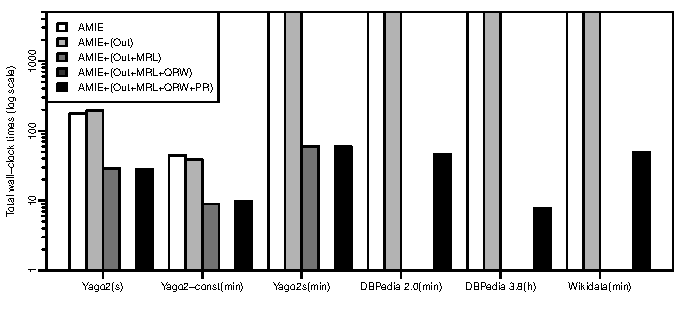
\includegraphics{figures/individual}
\caption{Performance of individual refinement improvements}
\label{individual}
\end{figure*}


% \begin{center}
% \begin{savenotes}
% \begin{table}[t]
% \footnotesize
% \centering
% \begin{tabular}{|l| r |r r|}
% \hline
% 			& \multicolumn{2}{c|}{AMIE (Conf $\ge 0.1$) }		& \multicolumn{2}{c|}{AMIE+(full)} 	\\ \cline{2-5}
% KB			& Rules 	& $\ge 0.1$		& Rules		& Prun. prec. 	   \\ \hline
%   YAGO2  		& 135		& 			& 68 		& 100.00\%      	    \\ 
%   YAGO2 (const)  	& 19132		& 			& 15634		& 100.00\% 	    \\  
%   YAGO2 ($l=4$)  	& 1382		&			& 645		& 100.00\%   	    \\ 
%   YAGO2s  		& 247*		&			& 94	 	& 100.00\%		    \\
%   DBpedia 2.0 		& 26812*	&			& 112865	& 98.26\%      	    \\ 
%   DBpedia 3.8 		& 4931*		&			& 5087       	& 98.41\%	    \\
%   Wikidata  		& 1244*		&			& 1650		& 96.93\%      	    \\  \hline
% \end{tabular}
% \caption{Output comparison of AMIE and AMIE+.\\ starred: output after processing for 1 day.}
% \label{outputComparison}
% \end{table}
% \end{savenotes}
% \end{center}

\begin{center}
\begin{savenotes}
\begin{table}[t]
\footnotesize
\centering
\begin{tabular}{|l| r |r r r|}
\hline
			& AMIE			& \multicolumn{3}{c|}{AMIE+(full)} 	\\ \cline{2-5}
KB			& Rules 		& Rules		&Pruned	& Prun. prec. 	   \\ \hline
  YAGO2  		& 68			& 68 		&24 	&100.00\%      	    \\ 
  YAGO2 (const)  	& 15634			& 15634		&24	&100.00\% 	    \\  
  YAGO2 ($l=4$)  	& 645			& 645		&203 	&100.00\%   	    \\ 
  YAGO2s  		& 94*			& 94	 	&78 	&100.00\%		    \\
  DBpedia 2.0 		& 24308*		& 112865	&5380 	&98.26\%      	    \\ 
  DBpedia 3.8 		& 2470*			& 5087       	&2621 	&98.41\%	    \\
  Wikidata  		& 746*			& 1650		&943 	&96.94\%      	    \\  \hline
\end{tabular}
\caption{Output comparison of AMIE (PCA conf $\ge$ 0.1) and AMIE+ full. Starred: output after processing for 1 day.}
\label{outputComparison}
\end{table}
\end{savenotes}
\end{center}



\paragraph{Output Comparison}
\comment{Fabian}{Shouldn't we run AMIE also with a confidence threshold of 0.1, just to have the two comparable? Anyway, a confidence threshold of 10\% makes sense... If so, change in several places in this paper.}
\comment{Done. Only for YAGO I rerun the experiments. For the other datasets I lie on the fact that the confidence threshold has a neglibible impact in AMIE's runtime.}
Table~\ref{outputComparison} shows a comparison of AMIE and AMIE+ in terms of output (number of rules).
For AMIE+ full we report the number of rules that were pruned by the confidence approximation.
To assess the quality of the confidence approximation, we report in addition the \emph{pruning precision}.
The pruning precision is the ratio of rules for which the confidence approximation introduced
in Section~\ref{sec:appr} overestimates the actual confidence. We
calculate this ratio by counting the number of times that the heuristics
produce a higher value than the real confidence (among the rules on which the approximation is applicable). 
For example, a pruning precision of 96\% means
that in 4\% of the cases the system erroneously pruned rules with a confidence higher than 0.1.
As in the previous section, we set a threshold of 0.1 PCA Confidence for AMIE. We also interrupted the system 
if it ran more than one day. In those cases, we report the output until the point of interruption (denoted by a ``*'' in Table~\ref{outputComparison}).
% Note that AMIE runs without any confidence threshold, while AMIE+ runs with confidence threshold of 0.1.
% Thus, we expect AMIE+ to output less rules than AMIE.
% However, if a system ran for more than one day, we interrupted it
% and considered the output until the point of interruption (denoted by a ``*'' in Table~\ref{outputComparison}).
This is particularly obvious for DBpedia 2.0, where AMIE found only 24K rules, while AMIE+(full) produces 112K rules.
This means that the values reported in Table~\ref{outputComparison}
may have been calculated on a
subset of all the rules, thus being an estimation of the actual pruning precision. 
As we can see, the speed-up provided by AMIE+(full) does not entail a serious decrease in the quality of the output: 
AMIE+ does not miss more than 4\% of the rules with confidence above 10\%.  

\comment{Fabian}{Several tables and graphs remain to be explained!}


\paragraph{Performance of confidence approximation w.r.t. to rule-length}
\comment{Fabian}{What is this? Will it be in the paper?}

\ignore{ %% this is luis version
Table~\ref{amievsplus} shows the runtimes of AMIE and AMIE+ with different setups on our test KBs.
%The different setups include: default AMIE+, AMIE+ with the PCA confidence
%bound enabled and AMIE+ with all the optimizations.
%If a system ran for more than one day without finishing, we interrupted it and reported the Fabian: said below
%output obtained until that point in time.
For AMIE, we show only the runtime. Since our goal is to observe the effect of each enhancement in the runtime of AMIE+, 
we show runtimes for combinations of the improvements introduced in Sections~\ref{subsec:lossless} and~\ref{subsec:speedingConfidenceEvaluation}. 
These includes:
\begin{enumerate}
 \item AMIE+ in its default configuration, i.e., with the lossless enhancements: MRL + QRW + PR. We refer to this setting as \emph{Default}.
 \item We investigate the effect of the confidence approximation by itself and call this setting \emph{AMIE+ with confidence approximation}.
 \item We incrementally add the lossless heuristics to the last setting, leading to three additional subsettings:
 \begin{enumerate}
  \item AMIE+ with confidence approximation + MLR
  \item AMIE+ with confidence approximation + MLR + QRW
  \item AMIE+ with confidence approximation + MLR + QRW + PR or simply \emph{Full AMIE+}
 \end{enumerate}
\end{enumerate}

We also report the number of rules produced in each setting. 
Since the lossless enhacements do not alter the output of AMIE, we report a single rule count for settings 2 and 3. 
To assess the quality of the confidence approximation, we report in addition the \emph{pruning precision}.
%In the default setting of AMIE+, the number of rules (and, in fact, the rules) are the same as in AMIE.
%with and without the confidence threshold.% (confidence thresholds do not alter runtime in AMIE).
% and when applicable the number
% of rules with PCA confidence equal or higher than the 10\% threshold.
% When the PCA confidence bound is enabled, we report
% the number of rules pruned by this heuristic. We do not report the number of rules,
% because this enhacement is lossless, that is, we obtain the same output as the default AMIE+ with a given confidence threshold.
%When all the optimizations are enabled, we additionally show the \emph{pruning precision}.
The pruning precision is the ratio of rules for which the confidence approximation introduced
in Section~\ref{sec:appr} overestimates the actual confidence. We
calculate this ratio by counting the number of times that the heuristics
produce a higher value than the real confidence (among the rules on which the approximation is applicable). 
For example, a pruning precision of 96\% means
that in 4\% of the cases the system erroneously pruned rules with a confidence higher than 0.1.
If a system ran for more than one day, we interrupted it
and considered the output until the point of interruption.
This means that the values reported in Table~\ref{amievsplus}
may have been calculated on a
subset of all the rules, thus being an estimation of the actual pruning precision.
This fact is particularly obvious
for DBpedia 2.0, where AMIE+ found only 14K rules without confidence threshold,
while AMIE+ with all the heuristics enabled produces 117K rules.

Table~\ref{amievsplus} shows that our enhancements have a significant impact in the runtime of AMIE.
On YAGO2, AMIE+ already exhibits a speedup factor of 6.7 w.r.t. AMIE.
For bigger and more complex datasets, however, even AMIE+  could not finish in one day. 
It is therefore required to enable all the optimizations to achieve reasonable runtimes.
We can also see that the confidence upper bounds by themselves do not allow us to scale to the size of YAGO2s, DBpedia, or Freebase.
For example, they can prune only 6 rules on YAGO2s.
This is because they are applicable to only a very restricted set of rules, namely those of the form $r(x,z) \wedge r(y,z) \Rightarrow r_h(x,y)$ or
$r(z,x) \wedge r(z,y) \Rightarrow r_h(x,y)$.
Therefore, we need to enable the confidence approximations in order to scale to these KBs.
This heuristic, however, comes with the additional cost of computing the
join cardinalities for every pair of relations in the KB, which can be very expensive for KBs with many relations, such as DBpedia or Freebase.
Nevertheless, it is run only once and, as the results show, it pays off.
On KBs where normal rule mining would have required more than a day, 
AMIE+ can run in a few hours or, in the worst case, over-night.
This speedup does not entail a serious decrease in the quality of the output: 
in the majority of datasets, AMIE+ does not miss any of the rules with confidence above 10\%. 
In the other datasets, it misses at most 4\% of them.
}

% \begin{center}
% \begin{savenotes}
% \begin{table*}[t]
% \footnotesize
% \begin{tabular}{|l|c|c|c|c|c|c|c|c|c|c|}
% \hline
% \multirow{3}{*}{KB} 	& \multirow{3}{*}{AMIE}  	& \multicolumn{9}{c|}{AMIE+} 	\\ \cline{3-11}
% 			&  				& \multicolumn{3}{c|}{Default}		& \multicolumn{2}{c}{Upper bounds} 	& \multicolumn{4}{|c|}{Upper bounds + approx.}\\ \cline{3-11}
% 			&  				& Time & Rules & $\ge$ 10\% 		& Time & Pruned 			& Time & Rules & Pruned & Prune prec. \\ \hline
% YAGO2  			& 3.62min  			& 31.71s & 135 & 68 			& 31.21s & 3 				& 32.34s& 68 & 24 & 100\%\\
% YAGO2(const) 		& 14.09min  			& 12.17min  & 19028 & 15526 		& 12.10min & 3 				& 12.17min & 15526 & 24 & 100\% \\
% YAGO2s  		& $>$ 1 day 			& $>$ 1 day & 249 & 95  		& $>$ 1 day & 6  			& 53.2min & 95 & 78 & 100\%\\
% DBpedia 2.0  		& $>$ 1 day 			& $>$ 1 day  & 14405  & 12805 		& $>$ 1 day & 808 			& 1.77h & 117163 & 5377 & 96\%\\
% DBpedia 3.8  		& $>$ 1 day  			& $>$ 1 day   & 4215 & 2106  		& $>$ 1 day & 292 			& 8.24h & 5193 & 2621 & 97\%\\
% Freebase 		& $>$ 1 day 			& $>$ 1 day & 182  & 131 		& $>$ 1 day & 5 			& 7.51min & 169 & 37 & 100\% \\ \hline
% \end{tabular}
% \caption{Runtime and output comparison between AMIE and AMIE+ on different KBs. Times smaller than one hour are averaged over 3 runs.}
% \label{amievsplus}
% \end{table*}
% \end{savenotes}
% \end{center}

\begin{center}
\begin{savenotes}
\begin{table*}[t]
\footnotesize
\begin{tabular}{|l|c|c|c|c|c|c|c|c|c|c|}
\hline
\multirow{3}{*}{KB} 	& \multirow{3}{*}{AMIE}  	& \multicolumn{9}{c|}{AMIE+} 	\\ \cline{3-11}
 			& 				& \multicolumn{2}{c|}{Default}	& \multicolumn{7}{c|}{AMIE + conf. approx}   \\ \cline{3-11}
			&  				&Runtime	& Rules 	& Runtime  & +MRL     &+QRW 	&+PR		& Full	   	   & Rules	& Prun. prec. 	   \\ \hline
  YAGO2  		& 3.17min  			&29.37s		& 135		& 2.82min  & 29.03s   &38.16s 	&2.80min  	& 28.19s	   & 135 	& 100\%      	    \\ \hline
  YAGO2 (const)  	& 37.57min  			&11.72min	& 19132		& 37.05min & 8.90min  &12.04min &36.48min  	& 9.93min	   & 15634	& 100\% 	    \\ \hline  
  YAGO2 ($l=4$)  	& 24.99min  			&9.49min	& 1382		& 26.48min & 8.65min  &15.69min &26.39min  	& 8.35min 	   & 645	& 100\%   	    \\ \hline
  YAGO2s  		& $>$ 1 day  			&$>$ 1 day	& 247		&$>$ 1 day & 1h 7min  &1h 12min*&$>$ 1 day  	& 59.38min	   & 94	 	& 100\%		    \\ \hline
  DBpedia 2.0  		& $>$ 1 day  			&$>$ 1 day	& 26812		&$>$ 1 day & 1h 3min  & -       &$>$ 1 day  	& 46.88min	   & 112865	& 98.26\%      	    \\ \hline
  DBpedia 3.8  		& $>$ 1 day  			&$>$ 1 day	& 4931		&14h 10min*& 6h 10min &7h 33min*&15h 6min*  	& 7h 46min 	   & 5087       & 98.41\%	    \\ \hline
  Wikidata  		& $>$ 1 day  			&$>$ 1 day	& 1244		&$>$ 1 day & 1h 14min &11h 4min*&-  		& 48.86min	   & 1650	& 96.93\%      	    \\ \hline

% YAGO2s  		& $>$ 1 day 			& $>$ 1 day & 249 & 95  		& $>$ 1 day & 6  			& 53.2min & 95 & 78 & 100\%\\
% DBpedia 2.0  		& $>$ 1 day 			& $>$ 1 day  & 14405  & 12805 		& $>$ 1 day & 808 			& 1.77h & 117163 & 5377 & 96\%\\
% DBpedia 3.8  		& $>$ 1 day  			& $>$ 1 day   & 4215 & 2106  		& $>$ 1 day & 292 			& 8.24h & 5193 & 2621 & 97\%\\
% Freebase 		& $>$ 1 day 			& $>$ 1 day & 182  & 131 		& $>$ 1 day & 5 			& 7.51min & 169 & 37 & 100\% \\ \hline
\end{tabular}
\caption{Runtime and output comparison between AMIE and AMIE+ on different KBs. }
\label{amievsplus}
\end{table*}
\end{savenotes}
\end{center}

% \ffigure{Table}{PCA_assumption_entities}{Categories of relations w.r.t. the validity of the PCA}{
% \begin{tabular}{p{2.3cm}|p{3cm}| p{2cm}}
% \centering{Category}	& Relation 			& \% of hits	\\
% \hline
% Functions   		&\emph{wasBornIn} 		& 96.67\\
% 			&\emph{diedIn} 			& 96.42\\
% 			&\emph{hasCapital}		& 93.33\\
% \hline
% Quasi- 			&\emph{hasCurrency}		& 75\\
% Functions		&\emph{hasOfficialLanguage} 	& 73.33\\
% 			&\emph{graduatedFrom} 		& 64.29\\
% 			&\emph{isCitizenOf} 		& 96.42\\
% 			&\emph{directed}$^{-1}$ 	& 90\\
% 			&\emph{hasAcademicAdvisor} 	& 88.89\\
% 			&\emph{created}$^{-1}$  	& 86.67\\
% 			&\emph{isLeaderOf} 		& 89.47\\
% 			&\emph{isPoliticianOf}		& 100\\
% 			&\emph{isAffiliatedTo}		& 89.47\\
% \hline
% Granularity 		&\emph{isLocatedIn}		& 50\\
% Differences		&\emph{livesIn}			& 20.83\\
% \hline
% Implicit 		&\emph{livesIn} 		& 20.83\\
% Assumptions		&&\\
% \hline
% Source  		&\emph{influences}$^{-1}$	& 34.78\\
% Incompleteness		&\emph{imports}			& 0\\
% 			&\emph{exports}			& 0\\
% 			&\emph{actedIn}$^{-1}$		& 0\\
% 			&\emph{worksAt}			& 89.66\\
% 			&\emph{hasMusicalRole}		& 22.22\\
% 			&\emph{dealsWith}		& 10\\
% % 			&\emph{isInterestedIn}$^{-1}$	& ?\\
% % 			&\emph{isKnownFor}$^{-1}$	& ?\\
% \hline
% Extraction 		&\emph{participatedIn}$^{-1}$	& 48.14\\
% Incompleteness		&\emph{isMarriedTo}		& 79.31\\
% 			&\emph{produced}$^{-1}$		& 56.67\\
% 			&\emph{actedIn}$^{-1}$		& 0\\
% 			&\emph{playsFor}		& 20\\
% 			&\emph{holdsPoliticalPosition}	& 26.67\\
% 			&\emph{hasChild}$^{-1}$		& 26.67\\
% 			&\emph{hasWonPrize}		& 31.03\\
% 			&\emph{dealsWith}		& 10\\
% 			&\emph{influences}$^{-1}$	& 34.78\\
% 			&\emph{hasMusicalRole} 		& 22.22\\
% \end{tabular}
% }

\begin{table}[t]
\begin{tabular}{p{2.3cm}|p{3cm}| p{2cm}}
\centering{Category}	& Relation 			& \% of hits	\\
\hline
Functions   		&\emph{wasBornIn} 		& 96.67\\
			&\emph{diedIn} 			& 96.42\\
			&\emph{hasCapital}		& 93.33\\
\hline
Quasi- 			&\emph{hasCurrency}		& 75\\
Functions		&\emph{hasOfficialLanguage} 	& 73.33\\
			&\emph{graduatedFrom} 		& 64.29\\
			&\emph{isCitizenOf} 		& 96.42\\
			&\emph{directed}$^{-1}$ 	& 90\\
			&\emph{hasAcademicAdvisor} 	& 88.89\\
			&\emph{created}$^{-1}$  	& 86.67\\
			&\emph{isLeaderOf} 		& 89.47\\
			&\emph{isPoliticianOf}		& 100\\
			&\emph{isAffiliatedTo}		& 89.47\\
\hline
Granularity 		&\emph{isLocatedIn}		& 50\\
Differences		&\emph{livesIn}			& 20.83\\
\hline
Implicit 		&\emph{livesIn} 		& 20.83\\
Assumptions		&&\\
\hline
Source  		&\emph{influences}$^{-1}$	& 34.78\\
Incompleteness		&\emph{imports}			& 0\\
			&\emph{exports}			& 0\\
			&\emph{actedIn}$^{-1}$		& 0\\
			&\emph{worksAt}			& 89.66\\
			&\emph{hasMusicalRole}		& 22.22\\
			&\emph{dealsWith}		& 10\\
% 			&\emph{isInterestedIn}$^{-1}$	& ?\\
% 			&\emph{isKnownFor}$^{-1}$	& ?\\
\hline
Extraction 		&\emph{participatedIn}$^{-1}$	& 48.14\\
Incompleteness		&\emph{isMarriedTo}		& 79.31\\
			&\emph{produced}$^{-1}$		& 56.67\\
			&\emph{actedIn}$^{-1}$		& 0\\
			&\emph{playsFor}		& 20\\
			&\emph{holdsPoliticalPosition}	& 26.67\\
			&\emph{hasChild}$^{-1}$		& 26.67\\
			&\emph{hasWonPrize}		& 31.03\\
			&\emph{dealsWith}		& 10\\
			&\emph{influences}$^{-1}$	& 34.78\\
			&\emph{hasMusicalRole} 		& 22.22\\
\end{tabular}
\caption{Categories of relations w.r.t. the validity of the PCA.}
\label{PCA_assumption_entities}
\end{table}




%%%%%%%%%%%%%%%%%%%%%%%%%%%%%%%%%%%%%%%%%%%%%%%

\subsection{AMIE vs. State-of-the-art Systems} \label{competitors}
\comment{chris}{this is just a summary. Usability stuff are out. Constants on different modes are out, etc. Please see if you are happy with the result}

In this section we present an overview of the comparison between AMIE and two state-of-the-art rule mining system that are publicly available:
WARMR~\cite{GoeVan02} and ALEPH~\cite{Muggleton:1996:LPD:647996.742465}. A more detailed description of these experiments can be found in~\cite{amie}.
We compare these system with AMIE in terms of runtime and quality of produced rules. For a detailed usability comparison please refer to~\cite{amie}.

\subsubsection{AMIE vs. WARMR}
WARMR is a system that unifies ILP and association rule mining. Similar to APRIORI algorithms~\cite{Agrawal:1996:FDA:257938.257975}, it performs a
breadth-first search in order to find frequent patterns.
It generates Datalog queries of the form ``$?-A_1,A_2,...,A_n$'',
where $A_i$ are logical atoms. WARMR applies a closed world assumption for assessing the quality of the produced rules.

\paragraph{Runtime}
For comparing WARMR with AMIE in terms of runtime, we tweaked AMIE to simulate WARMR's confidence measure.  
WARMR was not able to terminate on YAGO2 in a time period of 1 day. Therefore, we created a sample of YAGO2 
(see~\cite{amie} for information on how to sample a KB for rule-mining purposes).
In that sample, AMIE mined her rules in 7.91s seconds.
WARMR, in contrast, took 18 hours. Both systems were run with an absolute support threshold of 5 entities.

We also ran both systems in a mode that allows them to mine rules with constants. 
AMIE completed the task in 1.68 minutes on average. WARMR for all relations did not terminate in 3 days.
Therefore, we ran it only for the relations \textit{diedIn}, \textit{livesIn}, \textit{wasBornIn}, for which it took 48h. 
Table \ref{warmrruntime} summarizes the runtime results for WARMR, AMIE, and AMIE+. To make AMIE+ comparable, 
we run it without confidence threshold, therefore the reported runtime for AMIE+ uses only the enhacements for the refinement phase.
We conclude that AMIE is better suited for large KBs than WARMR.
This is because WARMR is an ILP algorithm written in a logic programming environment, 
which makes the evaluation of all candidate queries inefficient.\\

\begin{table}
\begin{tabular}{l|rr rr|}
Constants 	& WARMR 		& AMIE 		& AMIE+\\
\hline
 no 		& 18h 			& 6.02s 	& 2.59s \\
 yes 		& (48h) 	 	& 1.43min  	& 1.45min\\
\end{tabular}
\caption{Runtimes on YAGO2 sample}
\label{warmrruntime}
\end{table}


\paragraph{Results} After filtering out non-connected rules, WARMR mined 41 closed rules. 
AMIE+, in contrast, mined 74 closed rules, which included the ones mined by WARMR.
We checked back with the WARMR team and learned that for a given set of atoms $B_1, ... B_n$, 
WARMR will mine only one rule,
picking one of the atoms as head atom (e.g., $B_1 \wedge ... \wedge B_{n-1} \Rightarrow B_n$).
AMIE, in contrast, will mine one rule for each possible choice of head atom (as long as the thresholds are met).
In other words, AMIE with the standard support and confidence measures simulates WARMR, but mines more rules.
Furthermore, it runs orders of magnitude faster. 
Especially for large datasets for which the user would have needed to use complicated sampling schemes in order to use WARMR,
AMIE can be a very attractive alternative.
Even for smaller datasets with rules with constants, AMIE can provide results while WARMR cannot.
Moreover, AMIE comes with metrics that go beyond the standard confidence and the standard support.
We will show later that these improve the quality of the results.

\subsubsection{AMIE vs. ALEPH}

ALEPH is an ILP system that implements a variety of scoring functions for measuring a rule's quality. For our experiments we used the 
\emph{Positives-only} evaluation function~\cite{Muggleton:1996:LPD:647996.742465,usir1753}, 
which is the most interesting for our setting, since it does not require the existence of explicit negative examples.
It takes random facts as negative evidence, instead:
\[ Score := log(P)-log\frac{R+1}{Rsize+2}-\frac{L}{P} \]
Here, $P$ is the number of known true facts covered (KBtrue, or A resp., in Figure~\ref{fig:prediction}), $R$ is the number of random examples covered, 
$Rsize$ is the total number of randoms, and $L$ is the number of atoms in the rule. 
The intuition is that a good rule should cover many positive examples, and few or no randomly generated examples. This ensures
that the rule is not overly general. Furthermore, the rule should use as few atoms as possible, and thus achieve a high compression.



\paragraph{Runtime}
We ran AMIE, AMIE+ and ALEPH on YAGO2 \cite{yago2}. For ALEPH, we used the positive-only evaluation function with $Rsize=50$ 
and we considered only clauses that were able to explain at least 2 positive examples,
so that we will not get grounded facts as rules in the output.
For a fair comparison, we also instructed AMIE and AMIE+ to run with a support threshold of 2 facts.
We did not use any confidence threshold.
AMIE+ terminated in 3.76 minutes and found rules for all relations. 
ALEPH runs for one head relation at a time. For some relations (e.g.\emph{isPoliticianOf}),
it terminated in a few seconds.
For others, however, we had to abort the system after 1 day without results (Tables \ref{alephrun0} and \ref{alephrun1}).
For each relation, ALEPH treats one positive example at a time. Some examples need little processing time, others block the system for hours.
We could not figure out a way to choose examples in such a way that ALEPH runs faster.
Hence, we used the sample of YAGO2 that we created for WARMR.
Again, runtimes varied widely between relations (Table \ref{alephrun2}).
Some relations ran in a few seconds, others did not terminate in a day.
The runtimes with constants are similarly heterogeneous, with at least 7 relations not terminating in 1 day.

\begin{table}
\begin{tabular}{l|ccc}
KB & ALEPH & AMIE & AMIE+\\
\hline
YAGO2 full & 4.96s to $>$ 1 day & 4.41min & 3.76min\\
YAGO2 Sample & 0.05s to $>$ 1 day & 5.65s & 2.90s \\
\end{tabular}
\caption{Runtimes ALEPH vs. AMIE/AMIE+}
\label{alephrun0}
\end{table}
\begin{table}[t]
 \begin{tabular}{l|r}
Relations & Runtime\\
\hline
isPoliticianOf, hasCapital, hasCurrency & $<$ 5min\\
dealsWith, hasOfficialLanguage, imports & $<$ 5min\\
isInterested, hasMusicalRole & $<$19min\\
hasAcademicAdvisor, hasChild& $>$ 1 day\\
isMarriedTo, livesIn, worksAt, isLocatedIn& $>$ 1 day\\ %[-0.4cm]
\end{tabular}
\caption{Runtimes of ALEPH on YAGO2}
\label{alephrun1}
\end{table}
\begin{table}[t]
\begin{tabular}{l|r}
Relations & Runtime\\
\hline
diedIn, directed, hasAcademicAdvisor & $<$ 2min\\
graduatedFrom, isPoliticianOf, playsFor & $<$ 2min\\
wasBornIn, worksAt, isLeaderOf &  $<$ 2min\\
exports, livesIn, isCitizenOf & $<$ 1.4h\\
actedIn, produced, hasChild, isMarriedTo & $>$ 1 day\\ %[-0.4cm]
\end{tabular}
\caption{Runtimes of ALEPH on YAGO2 sample}
\label{alephrun2}
\end{table}

\paragraph{Results}
We compared the output of ALEPH with the positives-only evaluation function to the output of AMIE/AMIE+ using the PCA
confidence on the sample of YAGO2 used for the runtime experiments.
Recall that ALEPH requires more than one day for some relations, so we used only rules for which the head
relation runs in less than one day.
ALEPH mined 56 rules, while AMIE mined 302 rules.
We order the rules by decreasing score (ALEPH) and decreasing PCA confidence (AMIE).
Table \ref{alephres} shows the number of predictions and their total precision.
We show the aggregated values at the points where both approaches have produced around 3K, 5K, and 8K predictions.
AMIE's PCA confidence succeeds in sorting the rules roughly by descending precision, so that the initial rules have an extraordinary precision 
compared to ALEPH's.
AMIE needs more rules to produce the same number of predictions as ALEPH (but she also mines more).

\begin{table}
\begin{tabular}{l|rrr}
	    & Top $n$ & Predictions & Precision \\
 \hline
 Positives-only & 7 & 2997 & 27\% \\
 PCA Confidence & 12 & 2629 & 62\% \\
 \hline
 Positives-only & 9 & 5031 & 26\% \\
 PCA Confidence & 22 & 4512& 46\% \\
 \hline
 Positives-only & 17 & 8457 & 30\% \\
 PCA Confidence & 23 & 13927  & 43\% \\
\end{tabular}
\caption{PCA confidence vs. positives-only score: aggregated precision of rules mined on YAGO2 sample.}
\label{alephres}
\end{table}

We suspect that ALEPH's positives-only evaluation function manages to filter out overly general rules only to some extent.
The reason is that this measure ``guesses'' negative examples at random, whereas rules usually create false predictions in a non-random way.
Even if a rule produces many false predictions, the intersection of these false predictions and the random counterexamples may be very small.
Consider for example the rule $bornIn(x,y) \Rightarrow diedIn(x,y)$, which produces false predictions for example for persons who have moved
to a different place during their life.
By creating negative examples just by considering random person-location pairs,
we might not produce any case for which the rule will give a false prediction,
simply because such a negative example will have a relatively small probability to be generated.
% ALEPH will mine, e.g., \emph{livesIn}$(A,C),$\emph{isLocatedIn}$(C,B) \Rightarrow$ \emph{isPoliticianOf}$(A,B)$.
% The problem is that ALEPH generates counterexamples by randomly using valid constants for variables $A$ and $B$.
% Hence, the probability of creating a random example in which $B$ is the place of residence of the specific person $A$ is very low.\\

\paragraph{Summary}
Our experimental results show that AMIE can be up to 3 orders of magnitude faster
than other state-of-the-art systems, namely WARMR~\cite{GoeVan02} and ALEPH~\cite{Muggleton:1996:LPD:647996.742465}.
The PCA confidence was shown to rank productive and correct rules higher than other confidence metrics.


\subsection{Performance of the PCA Confidence} \label{experimentspca}
The Partial Completeness Assumption (PCA) says that if, for a given subject $s$ and a given relation $r$, the KB knows one object $o$ with $r(s,o)$, then the KB knows \emph{all} objects $o'$ with $r(s,o')$ (Sec.~\ref{sec:pca}). In this section, we investigate the validity of the PCA as an assumption to generate counter-examples
for rule mining. Moreover, we revisit the comparison between the standard and the PCA confidence
as a ranking metric for rules. We also show how the type information can increase the predictive precision of rules.

\subsubsection{PCA Evaluation}\label{pcaEvaluation}
The original AMIE paper used the PCA but it did not evaluate whether this assumption is true or not \cite{amie}.
Since the PCA is one of the basic ingredients of AMIE's mining model,
we wanted to know to what extent this assumption holds in a real-world KB.
For this purpose, we looked into each of the 31 relations between entities in YAGO2.
For each relation $r$, we randomly sampled 30 subjects.
For each subject $x$, we checked whether the KB knows all $y$ with $r(x,y)$. If the relation is more inverse functional than functional
($ifun(r) > fun(r)$, see Section~\ref{subsec:functions}), we considered $r^{-1}$ instead.

As a ground truth, we took the Wikipedia page of $x$ and what we could find on the Web by a search engine.
It is obvious that such an evaluation cannot be done strictly quantitatively.
For example, a person might have worked for a company, but this fact might appear nowhere on Wikipedia -- or even on the Web.
Or a musician might play 10 instruments at different levels of proficiency, but Wikipedia mentions only the 4 main instruments.
Even a search on the Web might not tell us that there are more than 4 instruments.
Therefore, we resorted to a qualitative analysis.
We analyzed each of the relations manually, and grouped the relations into categories.
Some relations fall into multiple categories.
Table~\ref{PCA_assumption_entities} shows, for each relation, the percentage of subjects in our sample for which the PCA holds.

\paragraph{Functions and Quasi-Functions} By definition, the PCA holds for functions. Our manual analysis, however, did not result in 100\% precision for functional relations in Table~\ref{PCA_assumption_entities}.
This is because our analysis also counts the cases where the KB contains bugs. If, for instance, YAGO knows the wrong place of death of a person, then there exists another value outside YAGO that is the right value. However the PCA would reject it. Hence, we count this case as a miss.

The PCA extends well to relations that are strictly speaking not functions, but that have a high functionality.
These are relations that usually have one object per subject, even though there could be several.
For example, a person can graduate from several universities, but most people graduate from a single university. We call these relations \emph{quasi-functions}.
The PCA worked very well also on these, and predicted completeness correctly for $73\%-100\%$
of the subjects under investigation. Since the PCA takes into account the direction of the functionality, the PCA also holds for quasi inverse-functional relations such as \emph{directed}.

\paragraph{Granularity Differences} Some relations, such as \emph{locatedIn} and \emph{livesIn}, hold between an entity and a geographical region.
In that case, the region can be given at the granularity of a city, a region, a country, or a continent.
Naturally, if YAGO contains one of these, the others are possible options. Hence, PCA fails and we found rather low precision values.
However, these cases could be addressed if one restricts the range of the relation (say, to cities).
With such a restriction, the relations become functions or quasi-functions, which lifts them into the category where the PCA works well.
% We plan to investigate this possibility in future work.
As we will see in Section ~\ref{subsubsec:std_vs_pca}, the use of types can significantly improve the performance of AMIE. 

\paragraph{Implicit Assumptions} Some statements can be inferred from the Wikipedia page even if the page does not mention them. % For instance, %\emph{livesIn} is incomplete ``in-purpose'' in the sense
People usually do not state information that can easily be inferred by what they have stated before
(following Grice's Maxim of quantity and manner~\cite{grice}). %\footnote{\url{http://www.usingenglish.com/articles/grices-conversational-maxims.html}}).
For example, if someone graduated from a university, people usually do not feel obliged to mention that this person used to live in the country
 in which the university is located,
because this can easily be inferred by the reader. Only less obvious residences will be explicitly mentioned. Therefore, the PCA does not always hold.
Note that rules such as $graduatedFrom(x,y)\Rightarrow livesIn(x,y)$ can only be mined if Grice's maxims are occasionally violated by the authors of the articles.
If the authors always follow the maxims, then such rules cannot be mined, because there are not even positive examples for which the rule holds (lack of support).
In the case of YAGO, the only relation that we found in this category is \emph{livesIn}.


\paragraph{Source Incompleteness} For many relations, the source itself (Wikipedia) is incomplete.
Usually, these relations have, for each subject, some objects that are undisputed.
For example, it is undisputed that Albert Einstein is interested in physics. However, these relations also have objects that are less important, disputed, or unknown.
For example, Albert Einstein might also be interested in music (he played the violin), but maybe also in pancakes.
These less prominent objects are a lot less likely to appear in Wikipedia, or indeed on any Web page.
Even if they do, we can never be sure whether there is not still something else that Einstein was interested in.
For these relations, the knowledge sources are often incomplete by nature.
For example, not every single product that a country imports and exports is explicitly mentioned.
Whether or not this poses a problem depends on the application.
If ground truth is defined as what is universally true, then source incompleteness is a problem.
If ground truth is the source of the KB (i.e., Wikipedia in this case), then source incompleteness is not an issue.



\paragraph{Extraction Incompleteness} For a large number of relations, the Wikipedia page contains more objects for a given subject than the KB.
These are cases where the extraction process was incomplete.
In the case of YAGO, this is due to a strong focus on accuracy,
which causes the extraction to discard any extracted fact that cannot be type checked or linked to an entity.
This class of relations is the most sensitive category for the PCA.
The success of the PCA will depend on how many relations and to what extent they are affected by incomplete extractions.

\paragraph{Discussion} In summary, our analysis shows that it depends on the nature of the relation and on its type signature whether the PCA holds or not.
 There are a large number of relations for which the PCA is reasonable.
These are not just functions and inverse functions, but also relations that exhibit a similar behavior.

For many other cases, the PCA does not hold. In these cases, AMIE will falsely assume that a rule is making incorrect predictions -- although, in reality,
the predictions might be correct.
Thus, when the PCA does not hold, AMIE will err on the side of caution.

At the same time, the PCA is not as restrictive as the closed world assumption (CWA):
the PCA admits that there can be facts that are true, but not known to the KB.
For example, if a person has a birth date, then both the CWA and PCA would not admit another birth date. However, if a person does not have a birth date, then the PCA will admit that there can be a birth date, while the CWA will assume that there cannot be a birth date. Thus, the PCA is more permissive than the CWA.
This encourages us to use the PCA for the definition of our confidence. In the following, we will show that this definition of confidence produces
 more predictive and more accurate rules than the standard confidence, which is based on the CWA.

%\subsubsection{Standard Confidence vs. PCA Confidence }
\subsubsection{Evaluation of the PCA Confidence.}
\label{subsubsec:std_vs_pca}
In the following, we revisit the comparison between the standard confidence 
and the PCA confidence from~\cite{amie}.
The evaluation is based on the number and precision of predictions of the most confident rules according to each metric.
We then compare these results with a naive inference approach where we exploit the type signatures of 
relations and the fact that multiple rules can lead to the same prediction. 

% Our discussion includes a comparison of their predictions as well as the results of our empirical
% evaluation of the PCA assumption.

\paragraph{Standard vs PCA confidence}
In~\cite{amie}, we conducted an experiment to compare the standard and the PCA confidence 
as scoring metrics for rules.
We ran AMIE with the default setting on the YAGO2 dataset. %It contains nearly 500K entities and 948K facts.
We sorted the rules first by descending PCA confidence, and then by descending standard confidence, and looked at the top rules.
For each rule, we evaluated the predictions beyond YAGO2, either by automatic verification in a
newer version of the KB (YAGO2s) or by manually checking them in Wikipedia.
The bottom curves of Figure \ref{finalshow} plot the aggregated predictions versus the aggregated precision for the standard and the PCA confidence.
The $n$-th dot from the left represents the total number of unique predictions and the total precision of these predictions, 
aggregated over the first $n$ rules.
As we see, ranking the rules by standard confidence is a very conservative approach:
It identifies rules with reasonable precision, but these do not produce many predictions.
Going down in the list of ranked rules, the rules produce more predictions -- but at lower precision. 
The top 30 rules produce 113K predictions at an aggregated precision of 34\%.
In contrast, if we rank the rules by PCA confidence, we quickly get large numbers of predictions. The top 10 rules already produce 135K predictions -- at a precision of 45\%.
The top 30 rules produce 3 times more predictions than the top 30 rules by standard confidence -- at comparable precision.
This is because the PCA confidence is less conservative than the standard confidence.

\begin{figure}
%\hspace*{-5ex}
%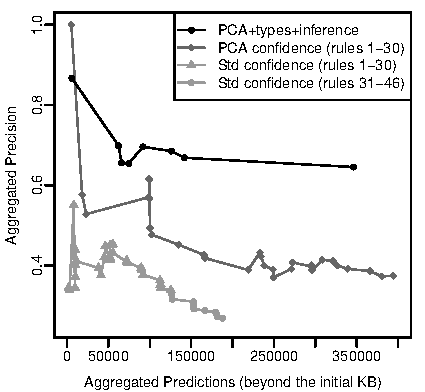
\includegraphics{figures/std_vs_pca}\ %\\[-0.5cm]
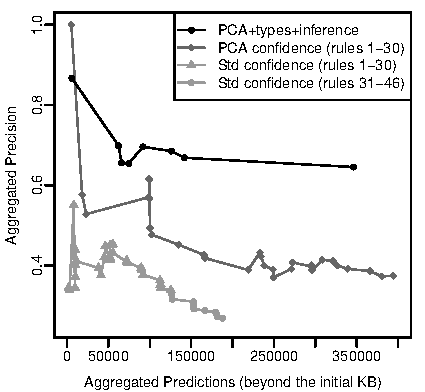
\includegraphics[width=0.5\textwidth]{figures/std_vs_pca}
\caption{Std. confidence vs. PCA confidence}
\label{finalshow}
\end{figure}

\paragraph{Using Type Information}
The naive prediction approach presented in~\cite{amie} was designed as a proof of concept 
to show the suitability of the PCA confidence as precision metric for rules mined on a Web-extracted KB. 
At the same time, a precision of 35\% is certainly not high enough to make actual predictions about the death place, future spouse, or future residence of a person. 

To make more accurate predictions, we have to combine these rules with more signals. In Section~\ref{PCA_assumption_entities} we discussed the granularity
differences in relations. For instance, the relation $livesIn$ is used to express a person's city or country of residence. 
This implies that, for example, the rule 
$livesIn(x, y) \Rightarrow isCitizenOf(x, y)$ can predict that some people are citizens of cities. Such spurious predictions decrease the precision
of the inference process.
Second, a prediction can be fired from multiple rules. If we consider rules as signals of evidence,  
then the more rules make a prediction, the higher its confidence should be and we should therefore prioritize it for evaluation.
In YAGO2, 9\% of the predictions are fired by more than one rule, when we use a confidence threshold of 0.1 PCA confidence. 

To account for the first observation, we configured AMIE to mine \emph{typed rules}. These have the form:
\[
 \vec{B} \wedge \textit{rdf:type}(x, D) \wedge \textit{rdf:type}(y, R) \Rightarrow r(x, y)
\]

\noindent where $D$ and $R$ correspond to the domain and range of the head relation $r$ in YAGO3\footnote{We used YAGO3 because the type signatures in older versions were too general for some relations.}. 
With a PCA confidence threshold of 0.1, AMIE found 57 typed rules on YAGO2.
This constraint suffices to solve the granularity differences discussed in Section~\ref{PCA_assumption_entities} as, for example, 
YAGO defines the relation $livesIn$ between people and cities.

To consider the second observation, we change the way predictions are ranked. In the original experimental setup, if 
multiple rules $R_1, \dots R_k$ made a prediction $p$, the prediction was only counted the first time it was fired. 
Since the rules were ranked by decreasing PCA confidence, 
this was equivalent to rank predictions according to their highest PCA confidence: 
\[
 score(p) := max\{conf_{pca}(R_1), \dots, conf_{pca}(R_k) \}
\]
We propose an alternative score instead:
\begin{equation}\label{predictions-score}
 score^*(p) := 1 - \prod_{i = 1}^{k}{(1 -conf_{pca}(R_i)})
\end{equation}
Equation~\ref{predictions-score} aggregates the PCA confidence of the rules so that the predictions concluded by multiple rules
are ranked higher. It also confers a probabilistic interpretation to the PCA confidence. The score of a prediction 
is the probabibility that at least one of the rules in $R_1, \dots R_k$ concludes $p$. This is computed as 1 minus the probabibility
that none of the rules concludes $p$. The probability of a rule not concluding $p$ is defined as 1 minus the PCA confidence of the rule.
The probabibility that none of the rules concludes $p$ is the product of the individual probabibilities.

We also note that Equation~\ref{predictions-score} assumes that rules are independent from each other. While this assumption may not be true sometimes, 
it still serves as a naive baseline for probabilistic inference methods. The upper curve in Figure~\ref{finalshow} shows the results
of our evaluation using typed rules and the naive independence score for predictions. We procedeed as in~\cite{amie}, that is,
we first used the rules to fire predictions, then we rank these predictions by descending score and computed their cumulative precision. 
Unlike the original experimental setup, the n-th point from the left in the new curve corresponds to the cumulative precision
of the predictions up to the n-th bucket. We bucketized the predictions by score using a bucket size of 0.1, i.e., the first point
corresponds to the predictions with score between 1 and 0.9, the next one accounts for the predictions with score between 0.9 and 0.8 and so on.

As we can observe, the type signatures have a significant effect in the precision of the predictions at the same level of recall of
the original experiment. The fact that we can achieve 60\% precision for 400K predictions, suggests that the PCA confidence in combination
with type checking are promising tool for more sophisticated rule-based inference approaches.  
While we should not add these predictions directly to a KB, we could send them to human evaluators to check their correctness.
It is much easier for a person to check fact candidates for their correctness than to invent them from scratch. 
In addition, this experimental setup could serve as a naive baseline for more sophisticated inference approaches.
%such a simple approach guarantees than more than a half of the predictions
% could be  it could still become a useful way
% a human evaluator
% could checked them The predicted candidates could be checked by a human before adding them to the KB. 
% It is much easier for a person to check fact candidates for their correctness than to invent them from scratch. 
% We will investigate this avenue of research in future work.

% While, such experimental
%  Nevertheless, this experimental setup could
%  serve as a naive baseline for more sophisticated inference approaches. In particular, the 
% predictions in KBs is 
% has been widely studied in the literature, however the experimental setup disregards two important characteristics of the data and the rule mining process.
% In 

% As we can see, the PCA confidence ranks predictive rules higher and is therefore more suitable for data prediction than the standard confidence.
% Nevertheless, rule mining with the PCA confidence achieves a cumulative precision in the range of 35\%-45\%.
% 
% This precision is certainly not high enough to make actual predictions about the death place, future spouse, or future residence of a person. However, such rules can still be useful for downstream applications. For example, if several rules predict the same fact, then this fact is more likely to be true. Hence, we could use our predictions to construct a probabilistic KB that weights each fact by the number of rules that predicted it. Facts with high cumulated confidence could be good candidates to populate KBs. 
% The predicted candidates could be checked by a human before adding them to the KB. It is much easier for a person to check fact candidates for their correctness than to invent them from scratch. We will investigate this avenue of research in future work.
% The predicted statements could also be used in ontology watermarking schemes such as in~\cite{DBLP:conf/www/SuchanekG12}. These schemes add plausible but wrong statements to the KB in order to mark it. Rule mining can deliver such statements.
% 
% We also note that our rules are insightful. Table \ref{rules} shows some of the rules that we mined.
% Being able to mine reasonable rules on semantic KBs of this size is an achievement beyond the current state of the art.

\ignore{
\begin{table}
\hspace*{-3.4ex}
\begin{tabular}{|l|}
\hline
\emph{isMarriedTo}$(x,y)\ \wedge$ \emph{livesIn}$(x,z) \Rightarrow $ \emph{livesIn}$(y,z)$\\
\emph{isCitizenOf}$(x,y) \Rightarrow$ \emph{livesIn}$(x,y)$\\
\emph{hasAdvisor}$(x,y)\ \wedge $ \emph{graduatedFrom}$(x,z) \Rightarrow$ \emph{worksAt}$(y,z)$\\
\emph{wasBornIn}$(x,y)\ \wedge$ \emph{isLocatedIn}$(y,z) \Rightarrow$ \emph{isCitizenOf}$(x,z)$\\
\emph{hasWonPrize}$(x,G.\;W.\;Leibniz) \Rightarrow$ \emph{livesIn}$(x,Germany)$\\
\emph{hasWonPrize}$(x,Grammy) \Rightarrow$ \emph{hasMusicalRole}$(x,Guitar)$\\
\hline
\end{tabular}
\caption{Several rules mined by AMIE}
\label{rules}
\end{table}
}
%\ignore{
% \paragraph{Precision of Mined Rules}
% In general, we can also use the confidence measures to estimate the actual precision of a rule.
% When mining rules, we are naturally interested in using an evaluation measure that correlates well with the real precision of a rule.
% To compare standard and PCA confidence, we ranked the mined rules by their actual precision.
% Table~\ref{cor-new} shows the average absolute error of the standard and PCA confidence weighted by the number of predictions produced by the rules based on the following formula:
% 
% \[
%  Error = \frac{\sum \limits_{r \in Output}{|Precision(r)-Conf(r)|\#Facts(r)}}{\sum \limits_{r \in Output}{\#Facts(r)}}
% \]
% %
% We observe that, on average, the PCA confidence estimates the precision of the rules better than the standard confidence.
% Thus, reasoning approaches can use the PCA confidence as a weight for the rule.
% 
% Note also that the PCA confidence is much closer to the actual precision value than the standard confidence for the top 20 rules.
% Since the error of PCA confidence is much smaller than the error of the standard confidence for the best performing rules (in terms of the actual precision),
% our results also imply that such rules have higher chances of being discovered during the mining process if we use the PCA confidence as quality evaluation metric.
% 
% 
% \begin{table}
% \small
% \begin{tabular}{l|ccc}
% 		& Top 20 rules 	&Top 30 rules	&All rules	\\
% \hline
% Confidence 	& 0.67		&0.49		&0.29 \\
% PCA Confidence 	& 0.28		&0.25		&0.28 \\
% \end{tabular}
% \caption{Average absolute prediction error (over new facts)}
% \label{cor-new}
% \end{table}
% }
% \begin{table}
% \begin{tabular}{l|rrr}
% 	    & Top $n$ & Predictions & Precision \\
%  \hline
%  Positives-only & 7 & 2997 & 27\% \\
%  PCA Confidence & 12 & 2629 & 62\% \\
%  \hline
%  Positives-only & 9 & 5031 & 26\% \\
%  PCA Confidence & 22 & 4512& 46\% \\
%  \hline
%  Positives-only & 17 & 8457 & 30\% \\
%  PCA Confidence & 23 & 13927  & 43\% \\
% \end{tabular}
% \caption{PCA confidence vs. positives-only score: aggregated precision of rules mined on YAGO2 sample.}
% \label{alephres}
% \end{table}

% \ignore{
% \subsubsection{PCA Confidence vs. Positives-Only Score}
% We compared the output of ALEPH with the positives-only evaluation function to the output of AMIE using the PCA
% confidence on the sample of YAGO2 used for the runtime experiments.
% Recall that ALEPH requires more than one day for some relations, so we used only rules for which the head
% relation runs in less than one day.
% ALEPH mined 56 rules, while AMIE mined 306 rules.
% We order the rules by decreasing score (ALEPH) and decreasing PCA confidence (AMIE).
% Table \ref{alephres} shows the number of predictions and their total precision.
% We show the aggregated values at the points where both approaches have produced around 3K, 5K, and 8K predictions.
% AMIE's PCA confidence succeeds in sorting the rules roughly by descending precision, so that the initial rules have an extraordinary precision compared to ALEPH's.
% AMIE needs more rules to produce the same number of predictions as ALEPH (but she also mines more).
% We suspect that ALEPH's positives-only evaluation function manages to filter out overly general rules only to some extent.
% ALEPH will mine, e.g., \emph{livesIn}$(A,C),$\emph{isLocatedIn}$(C,B) \Rightarrow$ \emph{isPoliticianOf}$(A,B)$.
% The problem is that ALEPH generates counterexamples by randomly using valid constants for variables $A$ and $B$.
% Hence, the probability of creating a random example in which $B$ is the place of residence of the specific person $A$ is very low.\\
% }







%%%%%%%%%%%%%%%%%%%%%%%%%%%%%%%%%%%%%%%%%%%%%%%%%%%%%%%%%%%%%%%%%%%%%%%%%%%%%%
%% previous version after this point


% \subsection{Overview}%\ \\[-0.7cm]
% \label{eval}
%
% \paragraph{Experiments}
% Before developing on the main experiments, we describe our datasets and
% experimental setup and provide a justification
% for the selection of rules up to 3 atoms. Then we describe our three main groups of experiments, where we
% (i) conduct an empirical evaluation of the PCA assumption on YAGO; (ii)
% compare AMIE and AMIE+ to two popular, state-of-the-art systems that are publicly available,
% WARMR~\cite{DehToi99,DehToi00} and ALEPH$^{\ref{foot:aleph}}$, and (iii) compare in detail
% the performance improvements of AMIE+ w.r.t AMIE.


% \paragraph{Settings} By default, AMIE uses a head coverage threhold of $\theta=1\%$ and
% ranks the resulting rules by decreasing PCA confidence. There is no need to deviate from this default configuration when a user runs AMIE.
% There are no parameters to tune. Moreover, AMIE+ inherits this default behavior and extends it by enabling the lossless optimizations (see Section~\ref{prunebound})
% in order to guarantee a faster execution without affecting the output.
% All experiments with AMIE/AMIE+ on all datasets are run in these settings, unless otherwise mentioned.
%
% \paragraph{Comparison with other systems} For some experiments, we want to compare AMIE's runtime and rule quality with other systems.
% To have an equal basis, we make AMIE
% simulate the metrics of the competitor systems.
% AMIE can threshold on support, head coverage, confidence, and PCA confidence, and she can rank by any of these.
% By default the system counts support on the two head variables, however it can also count on one of them. This variable can be
% always on the same position (e.g., always the subject) or can vary depending on the head relation. In that case, AMIE counts on the functional
% variable of the relation (see Section~\ref{subsec:functions} about functions).
% AMIE can also output non-closed rules. Since this is just a choice of what to output, it does not influence runtime.
% All experiments are run on a server with 48GB of RAM and 8 CPUs (Intel Xeon at 2.4GHz).
% We always mine rules without constants (i.e., without the instantiation operator), unless otherwise mentioned.
%
%
% \www{
% \paragraph{Knowledge Bases} We run our experiments on different KBs.
% In all cases, we removed the \emph{rdf:type} relationship, because it inflates the size of the KBs.
% We are aware that the \emph{rdf:type} relationship can be very helpful for rule mining.
% However, currently no approach (including ours) makes specific use of it.
% We plan to make use of it in future work. Furthermore, we removed all facts with literals (numbers and strings) from the KBs.
% Literal values (such as geographical coordinates) are shared by only very few entities, which makes them less interesting for rule mining.
% }
% Table~\ref{kbs} shows a summary of the KBs used for our experiments.
%
% \begin{savenotes}
% \ffigure{Table}{kbs}{Knowledge Bases used to test AMIE/AMIE+}{
% \footnotesize
% \begin{tabular}{l|c|c|c}
% KB & Facts & Subjects & Relations\\
% \hline
% YAGO2  & 948K & 470K & 32\\
% YAGO2s & 4.12M  & 1.65M & 37\\
% DBpedia 2.0 & 6.70M & 1.38M & 1595\footnote{This corresponds to the relations with more than 100 facts.} \\
% DBpedia 3.8 & 11.02M & 2.20M & 650 \\
% Freebase (people) & 8.92M & 2.07M & 51
% \end{tabular}
% }
% \end{savenotes}
%
% \subsection{Optimal length of rules}
% AMIE can in principle mine closed Horn rules with an arbitrary number of atoms, however all our experiments
% mine rules up to three atoms. This was decided from the observation than
% rules with more than three atoms are much more numerous and noisy. To support this assertion, we ran
% AMIE+ on YAGO2 with maximum rule length $n=4$ in order to investigate the quality of longer rules.
% Some of them are listed in Table~\ref{rules4atoms}. Let us look at one of the examples: \\
%
% {\small \raggedleft \emph{capital}$(a,f) \wedge$ \emph{hasGeoId}$(b,j) \wedge$ \emph{hasGeoId}$(f,j) \Rightarrow$ \emph{capital}$(a,b)$} \\
%
% It is easy to see that $f$ and $b$ bind always to the same values since the relations $hasCapital$ and $hasGeonamesId$ are
% highly functional. This makes the rule not interesting at all. Such kind of patterns arise because AMIE's
% language bias allows multiple atoms with the same relation. We could prune these type of rules by enforcing
% the constraint $f \neq b$ in the database, however inequality constraints
% come at expense of lower performance. We name these kind of rule patterns,
% \emph{subgraph redundant rules}%~\comment{Luis}{SOS: I cannot think of a better name}
% , since they contain groups of atoms (subgraphs) that bind to the same values
% and are thus redundant. We
% therefore tweaked AMIE to filter such cases. Another way to avoid these kind of rules, is to allow relations to appear
% at most once in each rule. We report running time and the number of rules mined by AMIE+
% with exactly 4 atoms with different settings in Table~\ref{yago4atoms}.
% The removal of subgraph redundant rules does not affect runtime because the rules are pruned after they are mined.
% %\comment{Chris}{in the rule or in the rule's body? Am I still able to get: you live where your spouse lives?}
% In contrast, avoiding repeated relations in atoms has a big impact in runtime and the size of the output.\\
%
% {\small
% \ffigure{Table}{rules4atoms}{Examples of high-confidence rules mined by AMIE with $n=4$ atoms}{
% \hspace*{-2.4ex}
% \begin{tabular}{|l|}
% \hline
% \emph{exports}$(b,h) \wedge$ \emph{imports}$(b,h) \wedge$ \emph{livesIn}$(a,b) \Rightarrow $ \emph{citizenOf}$(a,b)$\\
% \emph{capital}$(a,f) \wedge$ \emph{hasGeoId}$(b,j) \wedge$ \emph{hasGeoId}$(f,j) \Rightarrow$ \emph{capital}$(a,b)$ \\
% \emph{currency}$(j,b) \wedge$ \emph{isLeaderOf}$(i,e) \wedge$ \emph{livesIn}$(i,a) \Rightarrow $ \emph{currency}$(a,b)$\\
% \emph{diedIn}$(f,j) \wedge$ \emph{leaderOf}$(a,f) \wedge$ \emph{locatedIn}$(j,b) \Rightarrow $ \emph{politicianOf}$(a,b)$\\
% % \emph{hasOffLang}$(j,b) \wedge$ \emph{wasBornIn}$(e,a) \wedge$ \emph{wasBornIn}$(e,j) \Rightarrow $ \emph{hasOffLang}$(a,b)$\\
% \hline
% \end{tabular}
% }
% }
% \ffigure{Table}{yago4atoms}{AMIE on YAGO2 with maximum rule length $n=4$}{
% \small
% \begin{tabular}{l|c|c|}
% Setting & Runtime & Rules \\
% \hline
% Default & \multirow{2}{*}{5.71min} &  2144  \\
% No redundant subgraphs &  & 1231\\
% No repeated relations & 1.49min &  132 \\
% \end{tabular}
% }
%
% \paragraph{Discussion} Table~\ref{rules4atoms} shows some confident rules with 4 atoms. Our observations on the whole set of rules
% suggest that increasing the rule size does not provide a practical benefit: runtime increases as well as the number of uninteresting rules.
% Longer rules are also more complex to understand. The notion of length and complexity for hypotheses, is one of the key points of the
% Minimum Description Length principle, where among two hypotheses explaining the data comparably well, the simpler (shorter) is preferred.
% Furthermore, ILP approaches such as~\cite{Muggleton95inverseentailment} take into account this principle, giving preference to shorter rules.

% \begin{center}
% \begin{savenotes}
% \begin{table*}[t]
% \captionsetup{justification=centering, labelfont=bf}
% \setcounter{table}{\value{figureCounter}}
% \stepcounter{figureCounter}
% \footnotesize
% \begin{tabular}{|l|c|c|c|c|c|c|c|c|c|c|}
% \hline
% \multirow{3}{*}{KB} & \multirow{3}{*}{AMIE}  & \multicolumn{9}{c|}{AMIE+} \\ \cline{3-11}
%   &  & \multicolumn{3}{c}{Lossless}  & \multicolumn{2}{|c}{Upper bounds} & \multicolumn{4}{|c|}{Upper bounds + approx.}\\ \cline{3-11}
%   &  & Time & Rules & $\ge$ 10\% & Time & Pruned & Time & Rules & Pruned & Prune prec. \\ \hline
% YAGO2  & 3.62min  & 31.71s & 135 & 68 & 31.21s & 3 & 32.34s& 68 & 24 & 100\%\\
% YAGO2(const) & 14.09min  & 12.17min  & 19028 & 15526 & 12.10min & 3 & 12.17min & 15526 & 24 & 100\% \\
% YAGO2s  & $>$ 1 day & $>$ 1 day & 249 & 95  & $>$ 1 day & 6  & 53.2min & 95 & 78 & 100\%\\
% DBpedia 2.0  & $>$ 1 day & $>$ 1 day  & 14405  & 12805 & $>$ 1 day & 808 & 1.77h & 117163 & 5377 & 96\%\\
% DBpedia 3.8  & $>$ 1 day  & $>$ 1 day   & 4215 & 2106  & $>$ 1 day & 292 & 8.24h & 5193 & 2621 & 97\%\\
% Freebase & $>$ 1 day & $>$ 1 day & 182  & 131 & $>$ 1 day & 5 & 7.51min & 169 & 37 & 100\% \\ \hline
% \end{tabular}
% \centering\caption{\textbf{Runtime and output comparison between AMIE and AMIE+ on different KBs. Times smaller than one hour are averaged across 3 runs.}}
% \label{amievsplus}
% \end{table*}
% \end{savenotes}
% \end{center}

% \subsection{The PCA for Rule Mining}
%
% The PCA is the central assumption of AMIE's mining model. We conducted two rounds experiments to assess its feasibility.
% In the first round, we investigate how often the PCA holds in a web-extracted KB like YAGO, whereas in the second round
% we compare the performance of the PCA confidence against the standard confidence for data prediction under incompleteness.
%
% \subsubsection{PCA in Knowledge Bases}
% The PCA is the assumption that if a KB knows some values $r$-values for an entity $x$, then the entity does not have
% any other $r$-values. As discussed in Section~\ref{pcaEvaluation}, the PCA holds
% for functions and quasi-functions, whereas for other relations may be too optimistic
% about the completeness of the KB. Since the PCA is crucial in AMIE's mining model, we conducted an experiment
% to quantify how often it is wrong, that is, we estimated the ratio of cases when the KB did not know all
% the $r$-values of an entity. For this purpose, we constructed a sample of YAGO2s in
% in such a way that each relation occurs with 30 different random subjects. Then we
% verified for each pair entity-relation, whether the KB was actually complete.
% For instance, if YAGO knows about the two daughters of Barack Obama (i.e., Natasha and Malia) and there is no evidence about any other
% children in Wikipedia, the
% PCA is correct and this is counted as hit. On the contrary, if Wikipedia shows evidence about another child not present in YAGO,
% this counts as a miss. We show the percentage of hits per relation in Table~\ref{PCA_assumption}.

% \ffigure{Table}{PCA_assumption_entities}{Categories of relations w.r.t. the PCA}{
% \begin{tabular}{p{2cm}|p{5.4cm}}
% \centering{Category}		  & Relations 	\\
% \hline
% Functions   & \emph{wasBornIn}, \emph{diedIn}, \emph{hasCapital}\\%,  \comment{Chris}{have we evaluated those guys?} \comment{Luis: }{These relations do not exist in YAGO2, only in YAGO2s} \emph{happenedIn}, \emph{hasPredecessor}, \emph{owns}$^{-1}$ \\
% \hline
% Quasi-Functions & \emph{hasCurrency}, \emph{hasOfficialLanguage}, \emph{graduatedFrom}, \emph{isCitizenOf}, \emph{directed}$^{-1}$, \emph{hasAcademicAdvisor}, \emph{created}$^{-1}$,  \emph{isLeaderOf}, \emph{isPoliticianOf}\\%, \comment{Chris}{have we evaluated those guys?} \emph{wroteMusicFor}$^{-1}$\\
% \hline
% Granularity Differences& 	\emph{isLocatedIn},  \emph{livesIn}\\%,\comment{Chris}{have we evaluated those guys?} \emph{happenedIn}\\
% \hline
% Implicit Assumptions&\emph{livesIn} \\
% \hline
% Source Incompleteness & \emph{influences}$^{-1}$, \emph{imports}, \emph{exports}, \emph{actedIn}$^{-1}$, \emph{worksAt}, \emph{hasMusicalRole}, \emph{dealsWith}, \emph{isInterestedIn}$^{-1}$, \emph{isKnownFor}$^{-1}$\\
% \hline
% Extraction Incompleteness& \emph{participatedIn}$^{-1}$, \emph{isMarriedTo}, \emph{produced}$^{-1}$,  \emph{actedIn}$^{-1}$, \emph{playsFor}, \emph{holdsPoliticalPosition}, \emph{hasChild}$^{-1}$,  \emph{hasWonPrize}, \emph{dealsWith},\emph{influences}$^{-1}$, \emph{hasMusicalRole}\\
% \end{tabular}
% }

% \ffigure{Table}{PCA_assumption}{Ratio of cases the PCA is wrong for relations}{
% \begin{tabular}{p{2cm}|l|c}
% \textbf{Category} & \textbf{Relation} & \% of hits 	\\
% \hline
% % \multirow{3}{*}{Functions}  & $created^{-1}$	&77.78	\\
% %   & $diedIn$		&96.43	\\
% %   & $hasCapital$		&93.33	\\
% \multirow{9}{*}{\parbox{2cm}{{\small Quasi Functions}}}  &  $hasCurrency$&75	\\
% & $hasOfficialLanguage$	&73.33	\\
% & $graduatedFrom$	&64.29	\\
% & $isCitizenOf$		&96.42	\\
% & $directed^{-1}$	&90 	\\
% & $hasAcademicAdvisor$	&88.89	\\
% & $created^{-1}$	&86.67	\\
% & $isLeaderOf$		&89.47	\\
% & $isPoliticianOf$	&100	\\
% & $isAffiliatedTo$	&89.47 \\ \hline
% {\small Granularity differences} &   $isLocatedIn$	&50	\\ \hline
% {\small Implicit assumptions} & $livesIn$		&20.83	\\ \hline
% \multirow{5}{*}{\parbox{2cm}{{\footnotesize Source incompleteness}}} & $influences$		&34.78	\\
%    & $imports^{-1}$	&0	\\
%    & $actedIn^{-1}$	&0	\\
%    & $worksAt$		&89.66	\\
%    & $dealsWith$		&10\\ \hline
% \multirow{9}{*}{\parbox{2cm}{{\small Extraction incompleteness}}} &  $participatedIn^{-1}$	&48.14	\\
% & $isMarriedTo^{-1}$	&79.31	\\
% & $produced^{-1}$	&56.67	\\
% & $playsFor$		&20	\\
% & $produced^{-1}$	&56.67	\\
% & $holdsPoliticalPosition$	&26.67\\
% & $hasWonPrize$		&31.03\\
% & $hasChild^{-1}$	&26.67	\\
% & $hasWonPrize$		&31.03\\
%
% \end{tabular}
% }
% \comment{Luis}{We may group them according to the classification proposed in Section 4.4}
% \comment{Chris}{I agree. Perhaps we should just move this discussion in 4.4 (i.e. report the numbers there) or move 4.4 here.}
% We make use of the FUN-property of KBs (see Section~\ref{subsec:functions}), so that relations are always more functional than inverse functional in the
% evaluation. If this is not the case for a relation $r$, we use its inverse $r^{-1}$. This guarantees the evaluation of completeness goes always in the same direction: given
% a subject and a relation, we verify the completeness of the object values. We omitted functions such as $wasBornIn$
% in Table~\ref{PCA_assumption} since the PCA holds by definition for those relations. Some relations may fall within more than one category
% according to Section~\ref{pcaEvaluation} but we assign them to a single category in Table~\ref{PCA_assumption}
%
% \paragraph{Discussion}
% %Note that despite these problems, % Fabian: There is no problem, PCA is great! :-)
% We see that the PCA performs well in general in the rule mining scenario.
% This is true in particular if we compare it to the alternative, the Closed World Assumption (CWA).
% The CWA would reject all statements that are not in the KB.
% This includes the statements that the PCA assumes to be false. Thus, there are cases in which both assumptions err.
% For example, if the KB contains only one parent of a child, then both assumptions would (erroneously) reject an additional parent.
% One way to mitigate this, would be to learn an ``expected cardinality'' of a relation, and to reject as false everything
% that deviates too much from this cardinality.
% % \comment{Luis}{We should also consider the
% % standard deviation or maybe the whole probability distribution of the cardinality.}
% % This, however, would require coordination across rules if the number of objects in the KB falls more than 1 object short of the expected cardinality
% % -- something that we defer to future work.
% % \comment{Chris}{I didn't get it} \comment{Luis}{This is also not clear to me.}
% In all other cases, the PCA is more accurate than the CWA:
% The CWA will not admit a birthplace for a person that does not have a birthplace in the KB. The PCA will.
% Likewise, the CWA will not admit parents for a child that does not have parents in the KB, while the PCA does.
% This shows that the PCA is more careful when producing negative examples. This helps AMIE mine more productive rules,
% as we show in the next section.

% \subsection{Standard confidence vs. PCA confidence}
%
% In this section, we compare the standard confidence measure to the PCA confidence measure as ranking metric for rules.
% The comparison is based on the number and precision of predictions of the most confident rules according to each metric.
% % Our discussion includes a comparison of their predictions as well as the results of our empirical
% % evaluation of the PCA assumption.
%
% \subsubsection{Number of Predictions}
%
% We ran AMIE with the vanilla setting on the YAGO2 dataset. It contains nearly 500K entities and 948K facts.
% We sorted the rules first by descending PCA confidence, and then by descending standard confidence, and looked at the top rules.
% For each rule, we evaluated the predictions beyond YAGO2 %\comment{Katja}{Shouldn't it be ``beyond YAGO''?}\comment{Chris}{We train in Yago2, we test in yago2s. This is ok.}
% as described in Section \ref{eval}.
% Figure \ref{finalshow} plots the aggregated predictions versus the aggregated precision.
% The $n$-th dot from the left represents the total number of predictions and the total precision of these predictions, aggregated over the first $n$ rules.
% As we see, ranking the rules by standard confidence is a very conservative approach:
% It identifies rules with reasonable precision, but these do not produce many predictions.
% Going down in the list of ranked rules, the rules produce more predictions -- but at lower precision. The top 30 rules produce 113K predictions at an aggregated precision of 34\%.
% In contrast, if we rank the rules by PCA confidence, we quickly get large numbers of predictions. The top 10 rules already produce 135K predictions -- at a precision of 45\%.
% The top 30 rules produce 3 times more predictions than the top 30 rules by standard confidence -- at comparable precision.
% This is because the PCA confidence is less conservative than the standard confidence.
%
%
% \www{
% \ffigure{Figure}{finalshow}{Std. Confidence vs. PCA Confidence}{
% \hspace*{-5ex}
% 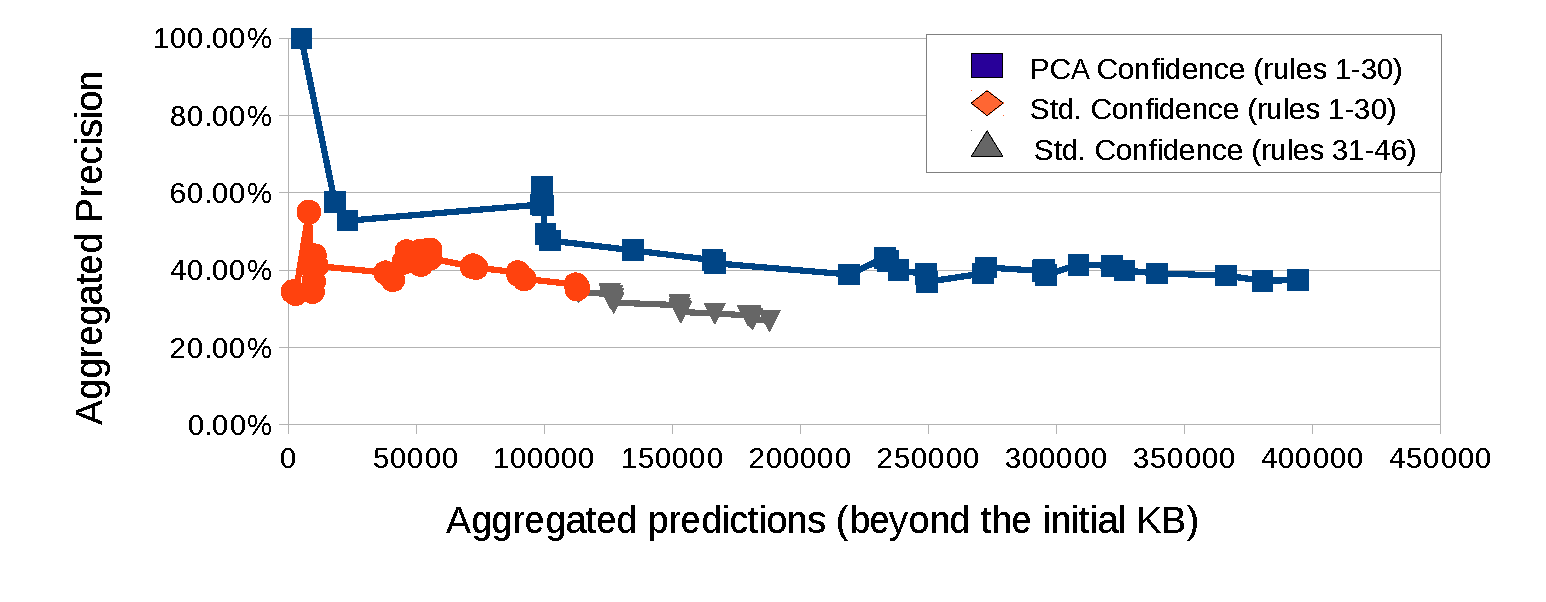
\includegraphics[scale=0.38]{figures/pca_vs_std_confidence.pdf}\ \\[-0.5cm]
% \comment{Katja}{Does anyone have a good idea how to increase readability of the chart? The green triangles are hard to distinguish from the red diamonds.}
% }
% }

% \paragraph{Discussion} The goal of the above experiment was to compare the quality of the rules that PCA confidence and standard confidence can mine.
% As we can see, the PCA confidence ranks predictive rules higher and is therefore more suitable for data prediction than the standard confidence.
% Nevertheless, rule mining with the PCA confidence achieves a cumulative precision in the range of 35\%-45\%. This happens because
% each rule by itself is imperfect.
% It is important to remark, however, that in a real life scenario where the quality of the derived facts matters,
% one should not just produce facts by deduction, like we did in this experiment. Rules should instead be used as building blocks
% for different applications. For example, while most of the predictions may not be true, they are still
% plausible statements that could be used in ontology watermarking schemes as in~\cite{conf/semweb/SuchanekGA11}.
% We can construct probabilistic KBs based on the predictions produced by the rules. For instance, multiple rules predicting the same fact,
% can have an additive effect on the confidence we have about that fact. Facts with high confidence are good candidates to populate KBs.
% If one wants to add those facts to the KB through a system that makes use
% of human agents, then reducing the number of potentially false predictions (i.e., facts with little statistical evidence)
% is a great advantage.


% \www{
% We also note that our rules are insightful. Table \ref{rules} shows some of the rules we mined. Being able to mine reasonable rules on semantic KBs of this size is an achievement beyond the current state of the art.\\
% }
%
% \www{
% \ffigure{Table}{rules}{Some Rules mined by AMIE}{
% \hspace*{-2.4ex}
% \begin{tabular}{|l|}
% \hline
% \emph{isMarriedTo}$(x,y) \wedge$ \emph{livesIn}$(x,z) \Rightarrow $ \emph{livesIn}$(y,z)$\\
% \emph{isCitizenOf}$(x,y) \Rightarrow$ \emph{livesIn}$(x,y)$\\
% \emph{hasAdvisor}$(x,y) \wedge $ \emph{graduatedFrom}$(x,z) \Rightarrow$ \emph{worksAt}$(y,z)$\\
% \emph{wasBornIn}$(x,y) \wedge$ \emph{isLocatedIn}$(y,z) \Rightarrow$ \emph{isCitizenOf}$(x,z)$\\
% \emph{hasWonPrize}$(x,G.\;W.\;Leibniz) \Rightarrow$ \emph{livesIn}$(x,Germany)$\\
% \emph{hasWonPrize}$(x,Grammy) \Rightarrow$ \emph{hasMusicalRole}$(x,Guitar)$\\
% \hline
% \end{tabular}
% }
% }


% \subsubsection{Precision of the Predictions}
% In general, we can also use the confidence measures to estimate the actual precision of a rule.
% When mining rules, we are naturally interested in using an evaluation measure that correlates well with the real precision of a rule.
% To compare standard and PCA confidence, we ranked the mined rules by their actual precision.
% Table~\ref{cor-new} shows the average absolute error of the standard and PCA confidence weighted by the number of predictions produced by the rules based on the following formula:
%
% \[
%  Error = \frac{\sum \limits_{r \in Output}{|Precision(r)-Conf(r)|\#Facts(r)}}{\sum \limits_{r \in Output}{\#Facts(r)}}
% \]
% %
% We observe that, on average, the PCA confidence estimates the precision of the rules better than the standard confidence.
% Thus, reasoning approaches can use the PCA confidence as a weight for the rule.
%
% Note also that PCA confidence is much closer to the actual precision value than the standard confidence for the top 20 rules. %\comment{Katja}{Maybe add the actual precision values to the table?}
% Since the error of PCA confidence is much smaller than the error of the standard confidence for the best performing rules (in terms of the actual precision),
% our results also imply that such rules have higher chance to be discovered during the mining process, if we use the PCA confidence as quality evaluation metric.
%
% \comment{Katja}{We will have to explain why the numbers here are so different from the WWW paper}
% \comment{Chris}{The evaluation is different (I think). We could point this out in the cover letter. My concern is more why we are converging in our errors with std conf.
% It means we screw up consistently whereas std confidence behaves very well at some point in the end.}
%
% \ffigure{Table}{cor-new}{Average Absolute Prediction Error \\(over new facts)}{
% \small
% \begin{tabular}{l|ccc}
% 		& Top 20 rules 	&Top 30 rules	&All rules	\\
% \hline
% Confidence 	& 0.67		&0.49		&0.29 \\
% PCA Confidence 	& 0.28		&0.25		&0.28 \\
% \end{tabular}
% }

% \subsection{AMIE vs. AMIE+}
% In this section we discuss the runtime improvements of AMIE+, which enable us to run on very large datasets.
% AMIE+ extends the original system AMIE with two types of enhacements:
%
% \paragraph{Lossless optimizations} They include Maximum Rule Length and Query Rewriting and Caching.
% These improvements do not alter the completeness of AMIE, i.e., they do not prune the output, but still allow for faster mining. AMIE+ enables them by default.
% \comment{Chris}{Why is confidence upper bound grouped as lossy optimization here? In the AMIE+ section it is under the lossless category. After all it
% is not an approximation.}
%
% \paragraph{Lossy optimizations} They include pruning by confidence upper bounds and by confidence approximations.
% These improvements might alter the output of AMIE since they prune rules that are expected to be low confident and very expensive to mine.
% Unlike the lossless heuristics, they require a minimum confidence threshold. For the type of rules discussed in Section~\ref{upperBound},
% the confidence upper bounds let us know precisely if the
% confidence of a rule will be below the confidence threshold, before calculating the actual confidence score. Our confidence
% approximations, on the other hand,
% provide a rough estimation of the confidence score which can be both an overestimation or underestimation of
% the actual confidence score. Underestimation affects the completeness of AMIE+,
% since some rules with high confidence score may be pruned. In any case, calculating the confidence upper bounds or estimating the confidence
% is much cheaper than computing the actuak confidence. All the experiments involving the lossy heuristics use a confidence
% threshold of 10\% PCA confidence.
%
%
% Table~\ref{amievsplus} shows the running times of AMIE and AMIE+ on our test KBs. For the latter, we display
% the running time with different configurations: default AMIE+ (i.e., only lossless heuristics enabled), AMIE+ with confidence
% bounds and AMIE+ with all the optimizations. If the system runs more than one day without finishing, we interrupted it and reported the
% output obtained until that point in time.
% For AMIE we show the runtime reported in~\cite{amie}. For the default configuration of AMIE+,
% we show the running time, the total number of rules
% and the number of rules with PCA confidence equal or higher than 10\%. Note that for
% all KBs except YAGO2, AMIE+ (only lossless heuristics enabled) could not finish in one day.
% The situation is not much different when we only enable the PCA confidence bounds with threshold 10\%. For this setup,
% we report the running time
% and the number of rules pruned by this heuristic. When all the optimizations are enabled, we report runtime, number of rules output, number of rules
% pruned by the heuristics and the pruning precision. The pruning precision is the ratio of rules for which the confidence approximation introduced
% in Sec.~\ref{subsec:pruningbyapprox} overestimates the actual confidence. We
% calculate this ratio by counting the number of times the heuristic produces a higher value than the real confidence in the set of rules output
% by AMIE+ (where the approximation is applicable) with the default setup within one day of running.
% \comment{Chris}{Why count the times that we overestimated confidence? in this cases we will not prune. We should count the cases that we underestimated confidence
% and pruned nice rules.}
% This means the value reported on Table~\ref{amievsplus}
% was calculated on a
% subset of all the rules and is actually an approximation of the pruning precision. This fact is particularly obvious
% for DBpedia 2.0 where AMIE+ found
% only 12K rules over the 10\% threshold, whereas enabling all the heuristics produces 117K rules
% \comment{Chris}{Are these rules in total or rules above 10\%? If it is the first let's compare it with the rules in total of AMIE+}.
%
%
% Table~\ref{amievsplus} shows that our enhancements have a significant impact on the systems runtime. On YAGO2 and even without the more aggresive lossy enhacements,
% AMIE+ exhibits a
% speedup of 6.7x with respect to AMIE. For bigger and more complex datasets, it is required to enable all the optimizations to achieve reasonable running times.
% We can also see that the confidence upper bounds by themselves do not allow us to scale to the size of YAGO2s, DBpedia or Freebase. For example they can prune only
% 6 rules on YAGO2s. This occurs because they are applicable to a very restricted set of rules; those of the form $r(x,z) \wedge r(y,z) \Rightarrow r_h(x,y)$ or
% $r(z,x) \wedge r(z,y) \Rightarrow r_h(x,y)$. Therefore, to scale we need to enable the confidence approximations.
% This heuristic, however, comes with the additional cost of computing the
% join cardinalities for every pair of relations in the KB, which can be very expensive for KBs with many relations such as DBpedia or Freebase.
% Nevertheless, it is run only once and, as the results show, it pays off.
% \comment{Chris}{Do we have perhaps the time needed for preprocessing for these datasets?
% We could report total time and preprocessing time and then this argument can also be seen in the table.}



% \subsection{AMIE vs. WARMR and ALEPH}
% \noindent In this section, we compare AMIE to WARMR and ALEPH. For each system, we conduct 3 experiments: We first compare the usability of the competitor system to AMIE.
% Then, we compare their runtimes with AMIE and AMIE+. Last, we compare their outputs.
%
% \subsubsection{AMIE vs. WARMR}
%
% \www{
% \paragraph{Usability} WARMR is a system that unifies ILP and association rule mining. Similar to APRIORI algorithms~\cite{Agrawal:1996:FDA:257938.257975}, it performs a
% breadth-first search in order to find frequent patterns.
% WARMR generates Datalog queries of the form ``$?-A_1,A_2,...,A_n$'',
% where $A_i$ are logical atoms.
% }
%
% \www{
% To discover frequent patterns (as in association rule mining), we need to have a notion of frequency. Given that WARMR considers queries as patterns and that queries can have variables,
% it is not immediately obvious what the frequency of a given query is. Therefore, the user needs to specify
% %define what is actually
% the predicate that is being counted by the system (the \textit{key predicate}).
% Since the key predicate determines what is counted, it is necessary that it is contained in all queries.
% For this reason, WARMR starts with having nothing but the key predicate in the body of the rule and then constructs more rules by adding more predicates.
% In the usual scenario of market basket analysis, the system counts customer transactions.
% In a scenario in which the database is a KB, one solution is to count entities.
% Therefore, we add a predicate \emph{entity}$(x)$, which we fill with all entities of the KB}. On the contrary, AMIE does not require such a trick.
%
% For WARMR, the user needs to provide specific information (called type declarations) about which predicates can be added to a query, which of their variables can be fresh (output mode),
% which should have already appeared in another atom (input mode)
% and which can be both (input/output mode). In other words, the user needs to define the language bias in terms of type and mode declarations.
% In order to stay as close as possible to AMIE's language bias, each relation should have at least one variable with input/output mode, so that fresh variables can be introduced in the rules.
% For functional or inverse functional relations, we declared subjects (objects) with an input mode and objects (subjects) with an input/output mode.
% %\comment{Luis}{Just to be sure 100\% sure, WARMR always starts with the key predicate, right? If yes, we should state it. }
% For relations that are not clearly functional or inverse functional (e.g. \emph{actedIn}, \emph{hasChild}) we declared both variables with input/output mode.
% According to the type declaration we used, the rules output by WARMR are neither necessarily closed nor connected.
% In general, WARMR does not differentiate between intermediate constructed rules (e.g. connected, but not closed) and final rules (e.g. closed).
% This means that the user needs to filter out the useful rules for his application from all the intermediate constructed rules.
% % Therefore, we had to filter out from the output non-interesting rules for our scenario rules . % Fabian: "non-interesting" sounds very subjective
% For the comparison with AMIE, we filtered out non-closed and non-connected rules.
%
% \www{
% WARMR is also able to mine rules with constants. The user can define which predicates and arguments should be instantiated with constants (we call this mode MODE1).
% WARMR then checks all the constants appearing in the facts of that specific predicate and argument and afterwards uses them in the queries.
% MODE1 naturally entails an increase of the branching factor in the search space and an explosion in the number of candidates that need to be evaluated.
% Alternatively, WARMR allows the user to set a maximum number of constants to be used for each predicate and argument (MODE2).
% Unfortunately, though, it does not provide a way for the user to influence the selection of these constants.
% In other words, there is no guarantee that the constants that WARMR will use are the most promising ones} in terms of support.
%
% \www{
% Thus, we conclude that the broader mission and the broader applicability of WARMR entails that much more configuration, acquaintance, and expert knowledge is needed to make it mine Horn rules on semantic KBs.
% }
%
% \www{
% \paragraph{Runtime}
% YAGO2\cite{yago2} contains around 940K facts about 470K entities.
% WARMR was not able to terminate on this data in a time period of 1 day. Therefore, we created a sample of YAGO2.
% Randomly selecting a number of facts from the initial dataset could break the interesting links between the entities.
% Therefore, we randomly selected 10,000 seed entities and included their 3-hop neighborhood.
% This yielded 14K entities and 47K facts.
% This sample contains all available information in a radius of 3 hops around the seed entities, but much less information about the entities at the periphery of the subgraph.
% Therefore, we restricted the values for the key predicate
% to the seed entities only.
% }
%
% Since the sample is much smaller than the original KB, we lowered the support threshold to 5 entities.
% In order to make AMIE and WARMR comparable, we tweaked AMIE so that she will also count seed entities while calculating the standard confidence.
% We ran AMIE with the same parameters on the sample. AMIE mined her rules in 7.91s seconds on average across 3 runs.
% WARMR, in contrast, took 18 hours.
% We also ran both systems allowing them to mine rules with constants. AMIE completed the task in 1.68 minutes on average. WARMR in MODE1 for all relations did not terminate in 3 days.
% Therefore, we ran it also only for the relations \textit{diedIn}, \textit{livesIn}, \textit{wasBornIn}, for which it took 48h. We also ran WARMR in MODE2.
% To have reasonable runtimes, we allowed WARMR to find constants only for one predicate (\emph{diedIn}). We also restricted it to find only 20 constants. WARMR ran 19 hours.
% Table \ref{warmrruntime} summarizes the runtime results for WARMR, AMIE and AMIE+. We conclude that AMIE is better suited for large KBs than WARMR.
% This is because WARMR is an ILP algorithm written in a logic programming environment, which makes the evaluation of all candidate queries inefficient.\\
%
% \ffigure{Table}{warmrruntime}{Runtimes on YAGO2 sample}{
% \footnotesize
% \begin{tabular}{l|rr rr|}
% Constants & WARMR & AMIE & AMIE+\\
% \hline
%  no & 18h & 7.91s & 5.24s \\
%  yes & (48h) / (19.3h) & 1.68min  & 1.06min\\
% \end{tabular}
% }
%
% \www{
% \paragraph{Results} After filtering out non-connected rules, WARMR mined 41 closed rules. AMIE+, in contrast, mined 207 closed rules, which included the ones mined by WARMR.
% We checked back with the WARMR team and learned that for a given set of atoms $B_1, ... B_n$, WARMR will mine only one rule, picking one of the atoms as head atom (e.g., $B_1 \wedge ... \wedge B_{n-1} \Rightarrow B_n$).
% AMIE, in contrast, will mine one rule for each possible choice of head atom (as long as the thresholds are met). In other words, AMIE with the standard support and confidence measures simulates WARMR, but mines more rules.
% Furthermore, it runs orders of magnitude faster. Especially for large datasets for which the user would have needed to use complicated sampling schemes in order to use WARMR, AMIE can be a very attractive alternative.
% Even for smaller datasets with rules with constants, AMIE can provide results while WARMR cannot. Moreover, AMIE comes with metrics that go beyond the standard confidence and the standard support.
% We will show later that these improve the quality of the results.
% }
%
% \www{
% \subsubsection{AMIE vs. ALEPH}
%
% \paragraph{Usability} ALEPH can be run with different commands that influence the search strategy. We chose the \emph{induce} command, which runs fastest.
% For running ALEPH, the user has to specify the target predicate for learning (the head predicate of the rules).
% In the following, we ran ALEPH successively with all predicates of the KB as targets.
% In addition, the user has to specify a series of type and mode declarations (similar to WARMR), which will be used as a language bias in order to restrict the search space.
% In addition, the user needs to provide ALEPH with files containing the background knowledge and positive examples for the target predicate.
% In contrast, AMIE requires no such input. It will run on a KB without any prespecified choices of predicates.\\
% }
%
%
% \ffigure{Table}{alephrun0}{Runtimes ALEPH vs. AMIE/AMIE+}{
% \footnotesize
% \begin{tabular}{l|ccc}
% KB & ALEPH & AMIE & AMIE+\\
% \hline
% YAGO2 full & 4.96s to $>$ 1 day & 3.62min & 1.62min\\
% YAGO2 Sample & 0.05s to $>$ 1 day & 7.91s & 2.27s \\
% \end{tabular}
% }
%
% \www{
% \ffigure{Table}{alephrun1}{Runtimes of ALEPH on YAGO2}{ % no constants
% %\begin{flushleft}
% \begin{tabular}{l|r}
% Relations & Runtime\\
% \hline
% isPoliticianOf, hasCapital, hasCurrency & $<$ 5min\\
% dealsWith, hasOfficialLanguage, imports & $<$ 5min\\
% isInterested, hasMusicalRole & $<$19min\\
% hasAcademicAdvisor, hasChild& $>$ 1 day\\
% isMarriedTo, livesIn, worksAt, isLocatedIn& $>$ 1 day\\ %[-0.4cm]
% \end{tabular}
% %\end{flushleft}
% } %\ \\[-1cm]
%
% \ffigure{Table}{alephrun2}{Runtimes of ALEPH on YAGO2 sample}{
% %\begin{flushleft}
% \begin{tabular}{l|r}
% Relations & Runtime\\
% \hline
% diedIn, directed, hasAcademicAdvisor & $<$ 2min\\
% graduatedFrom, isPoliticianOf, playsFor & $<$ 2min\\
% wasBornIn, worksAt, isLeaderOf &  $<$ 2min\\
% exports, livesIn, isCitizenOf & $<$ 1.4h\\
% actedIn, produced, hasChild, isMarriedTo & $>$ 1 day\\ %[-0.4cm]
% \end{tabular}
% %\end{flushleft}
% }%\ \\[-1cm]
% }
%
% \www{
% \paragraph{Runtime}
% We ran AMIE and ALEPH on YAGO2 \cite{yago2}. For ALEPH, we used the positive-only evaluation function with $Rsize=50$ and we considered only clauses that were able to explain at least 2 positive examples,
% so that we will not get grounded facts as rules in the output.
% For a fair comparison, we also instructed AMIE to run with a support threshold of 2 facts.
% AMIE terminated in 3.62 minutes, and found rules for all relations. ALEPH ran for one head relation at a time. For some relations (e.g.\emph{isPoliticianOf}),
% it terminated in a few seconds.
% For others, however, we had to abort the system after 1 day without results (Tables \ref{alephrun0} and \ref{alephrun1}).
% For each relation, ALEPH treats one positive example at a time. Some examples need little processing time, others block the system for hours.
% We could not figure out a way to choose examples in such a way that ALEPH runs faster.
% Hence, we used the sample of YAGO2 that we created for WARMR.
% %, which contains around 47k facts for a variety of target predicates.
% Again, runtimes varied widely between relations (Table \ref{alephrun2}).
% Some relations ran in a few seconds, others did not terminate in a day.
% The runtimes with constants are similarly heterogeneous, with at least 7 relations not terminating in 1 day.
% }
%
% \paragraph{Results}
% We compared the output of ALEPH on the head relations for which it terminated to the output of AMIE on these head relations, on the sample dataset.
% ALEPH mined 56 rules, while AMIE mined 306 rules.
% We order the rules by decreasing score (ALEPH) and decreasing PCA confidence (AMIE).
% Table \ref{alephres} shows the number of predictions, and their total precision as described in Section \ref{eval}.
% We show the aggregated values at the points where both approaches have produced around 3K, 5K, and 8K predictions.
% AMIE's PCA confidence succeeds in sorting the rules roughly by descending precision, so that the initial rules have an extraordinary precision compared to ALEPH's.
% AMIE needs more rules to produce the same number of predictions as ALEPH (but she also mines more).
% We suspect that ALEPH's positives-only evaluation function manages to filter out overly general rules only to some extent.
% ALEPH will mine, e.g., \emph{livesIn}$(A,C),$\emph{isLocatedIn}$(C,B) \Rightarrow$ \emph{isPoliticianOf}$(A,B)$.
% The problem is that ALEPH generates counterexamples by randomly using valid constants for variables $A$ and $B$.
% This means that the probability of creating a random example in which $B$ is the place of residence of the specific person $A$ is very low.\\
%
% \ffigure{Table}{alephres}{Top Rules of ALEPH vs. AMIE on YAGO2 sample}{
% \begin{tabular}{l|rrr}
%  System & Top $n$ & Predictions & Precision \\
%  \hline
%  ALEPH & 7 & 2997 & 27\% \\
%  AMIE & 12 & 2629 & 62\% \\
%  \hline
%  ALEPH & 9 & 5031 & 26\% \\
%  AMIE & 22 & 4512& 46\% \\
%  \hline
%  ALEPH & 17 & 8457 & 30\% \\
%  AMIE & 23 & 13927  & 43\% \\
% \end{tabular}
% }
%
%
%
%
%
%
% \subsection{AMIE for Data Prediction}
% As a simple proof of concept, we ran AMIE on older versions of YAGO (YAGO2)\cite{yago2} and DBpedia (2.0)\cite{dbpedia}
% and used to the rules to make predictions which we verified in newer versions of the KBs, YAGO2s and DBpedia 3.8.
% We report in Table~\ref{dbp} the number of predicted facts that are in the newer version of the KB but not in the old one (hits).
% A fact can be predicted by multiple rules, so we report the count with and without duplicates.
% The results show that logical rules can be used to generate
% a large number of plausible facts. Moreover, evidence from multiple rules can increase
% the confidence we have on a fact. This suggests a potential for the development of more sophisticated models
% to estimate the accuracy of our precisions and identify facts that are more likely true, either now or in the future.
% We leave the exploration of this avenue as future work. \\
%
% \ffigure{Table}{dbp}{AMIE for predicting facts on YAGO and DBpedia}{
% \small
% \begin{tabular}{l|c|cc|}
% Old dataset & Rules & Total hits & Unique Hits \\
% \hline
% YAGO2 & 135   & 14K  & 12K \\
% YAGO2 (const) & 19028   & 79K & 17K\\
% DBpedia 2.0 & 117163  & - & \\
% \end{tabular}
% }

